%----------------------------------------------------------------------------------------
%	PACKAGES AND OTHER DOCUMENT CONFIGURATIONS
%----------------------------------------------------------------------------------------

\documentclass{tufte-book} % Use the tufte-book class which in turn uses the tufte-common class
\usepackage{amssymb}
\usepackage{hyperref}
\usepackage{tcolorbox}

%\hypersetup{colorlinks} % Comment this line if you don't wish to have colored links

\usepackage{microtype} % Improves character and word spacing
\usepackage{booktabs} % Better horizontal rules in tables

\usepackage{graphicx} % Needed to insert images into the document
\graphicspath{{graphics/}} % Sets the default location of pictures
\setkeys{Gin}{width=\linewidth,totalheight=\textheight,keepaspectratio} % Improves figure scaling

\usepackage{fancyvrb} % Allows customization of verbatim environments

\fvset{fontsize=\normalsize} % The font size of all verbatim text can be changed here

\newcommand{\hangp}[1]{\makebox[0pt][r]{(}#1\makebox[0pt][l]{)}} % New command to create parentheses around text in tables which take up no horizontal space - this improves column spacing
\newcommand{\hangstar}{\makebox[0pt][l]{*}} % New command to create asterisks in tables which take up no horizontal space - this improves column spacing

\usepackage{xspace} % Used for printing a trailing space better than using a tilde (~) using the \xspace command

\newcommand{\monthyear}{\ifcase\month\or January\or February\or March\or April\or May\or June\or July\or August\or September\or October\or November\or December\fi\space\number\year} % A command to print the current month and year

\newcommand{\openepigraph}[2]{ % This block sets up a command for printing an epigraph with 2 arguments - the quote and the author
\begin{fullwidth}
\sffamily\large
\begin{doublespace}
\noindent\allcaps{#1}\\ % The quote
\noindent\allcaps{#2} % The author
\end{doublespace}
\end{fullwidth}
}

\newcommand{\blankpage}{\newpage\hbox{}\thispagestyle{empty}\newpage} % Command to insert a blank page

\usepackage{units} % Used for printing standard units

\newcommand{\hlred}[1]{\textcolor{Maroon}{#1}} % Print text in maroon
\newcommand{\hangleft}[1]{\makebox[0pt][r]{#1}} % Used for printing commands in the index, moves the slash left so the command name aligns with the rest of the text in the index 
\newcommand{\hairsp}{\hspace{1pt}} % Command to print a very short space
\newcommand{\ie}{\textit{i.\hairsp{}e.}\xspace} % Command to print i.e.
\newcommand{\eg}{\textit{e.\hairsp{}g.}\xspace} % Command to print e.g.
\newcommand{\na}{\quad--} % Used in tables for N/A cells
\newcommand{\measure}[3]{#1/#2$\times$\unit[#3]{pc}} % Typesets the font size, leading, and measure in the form of: 10/12x26 pc.
\newcommand{\tuftebs}{\symbol{'134}} % Command to print a backslash in tt type in OT1/T1

\providecommand{\XeLaTeX}{X\lower.5ex\hbox{\kern-0.15em\reflectbox{E}}\kern-0.1em\LaTeX}
\newcommand{\tXeLaTeX}{\XeLaTeX\index{XeLaTeX@\protect\XeLaTeX}} % Command to print the XeLaTeX logo while simultaneously adding the position to the index

\newcommand{\doccmdnoindex}[2][]{\texttt{\tuftebs#2}} % Command to print a command in texttt with a backslash of tt type without inserting the command into the index

\newcommand{\doccmddef}[2][]{\hlred{\texttt{\tuftebs#2}}\label{cmd:#2}\ifthenelse{\isempty{#1}} % Command to define a command in red and add it to the index
{ % If no package is specified, add the command to the index
\index{#2 command@\protect\hangleft{\texttt{\tuftebs}}\texttt{#2}}% Command name
}
{ % If a package is also specified as a second argument, add the command and package to the index
\index{#2 command@\protect\hangleft{\texttt{\tuftebs}}\texttt{#2} (\texttt{#1} package)}% Command name
\index{#1 package@\texttt{#1} package}\index{packages!#1@\texttt{#1}}% Package name
}}

\newcommand{\doccmd}[2][]{% Command to define a command and add it to the index
\texttt{\tuftebs#2}%
\ifthenelse{\isempty{#1}}% If no package is specified, add the command to the index
{%
\index{#2 command@\protect\hangleft{\texttt{\tuftebs}}\texttt{#2}}% Command name
}
{%
\index{#2 command@\protect\hangleft{\texttt{\tuftebs}}\texttt{#2} (\texttt{#1} package)}% Command name
\index{#1 package@\texttt{#1} package}\index{packages!#1@\texttt{#1}}% Package name
}}

% A bunch of new commands to print commands, arguments, environments, classes, etc within the text using the correct formatting
\newcommand{\docopt}[1]{\ensuremath{\langle}\textrm{\textit{#1}}\ensuremath{\rangle}}
\newcommand{\docarg}[1]{\textrm{\textit{#1}}}
\newenvironment{docspec}{\begin{quotation}\ttfamily\parskip0pt\parindent0pt\ignorespaces}{\end{quotation}}
\newcommand{\docenv}[1]{\texttt{#1}\index{#1 environment@\texttt{#1} environment}\index{environments!#1@\texttt{#1}}}
\newcommand{\docenvdef}[1]{\hlred{\texttt{#1}}\label{env:#1}\index{#1 environment@\texttt{#1} environment}\index{environments!#1@\texttt{#1}}}
\newcommand{\docpkg}[1]{\texttt{#1}\index{#1 package@\texttt{#1} package}\index{packages!#1@\texttt{#1}}}
\newcommand{\doccls}[1]{\texttt{#1}}
\newcommand{\docclsopt}[1]{\texttt{#1}\index{#1 class option@\texttt{#1} class option}\index{class options!#1@\texttt{#1}}}
\newcommand{\docclsoptdef}[1]{\hlred{\texttt{#1}}\label{clsopt:#1}\index{#1 class option@\texttt{#1} class option}\index{class options!#1@\texttt{#1}}}
\newcommand{\docmsg}[2]{\bigskip\begin{fullwidth}\noindent\ttfamily#1\end{fullwidth}\medskip\par\noindent#2}
\newcommand{\docfilehook}[2]{\texttt{#1}\index{file hooks!#2}\index{#1@\texttt{#1}}}
\newcommand{\doccounter}[1]{\texttt{#1}\index{#1 counter@\texttt{#1} counter}}

\usepackage{makeidx} % Used to generate the index
\makeindex % Generate the index which is printed at the end of the document

% This block contains a number of shortcuts used throughout the book
\newcommand{\vdqi}{\textit{VDQI}\xspace}
\newcommand{\ei}{\textit{EI}\xspace}
\newcommand{\ve}{\textit{VE}\xspace}
\newcommand{\be}{\textit{BE}\xspace}
\newcommand{\VDQI}{\textit{The Visual Display of Quantitative Information}\xspace}
\newcommand{\EI}{\textit{Envisioning Information}\xspace}
\newcommand{\VE}{\textit{Visual Explanations}\xspace}
\newcommand{\BE}{\textit{Beautiful Evidence}\xspace}
\newcommand{\TL}{Tufte-\LaTeX\xspace}

%----------------------------------------------------------------------------------------
%	BOOK META-INFORMATION
%----------------------------------------------------------------------------------------

\title{Practical Statistics} % Title of the book

\author[Diman Todorov]{Diman Todorov} % Author

\publisher{Counter Culture Labs} % Publisher

%----------------------------------------------------------------------------------------

\begin{document}

\frontmatter

%----------------------------------------------------------------------------------------
%	EPIGRAPH
%----------------------------------------------------------------------------------------

%\thispagestyle{empty}
%\openepigraph{It is not knowledge, but the act of learning, not possession but the act of getting there, which grants the greatest enjoyment.}{Carl Friedrich Gauss, {\itshape Letter to Bolyai, 1808}}
%\vfill
%\openepigraph{A designer knows that he has achieved perfection not when there is nothing left to add, but when there is nothing left to take away.}{Antoine de Saint-Exup\'{e}ry}
%\vfill
%\openepigraph{\ldots the designer of a new system must not only be the implementor and the first large-scale user; the designer should also write the first user manual\ldots If I had not participated fully in all these activities, literally hundreds of improvements would never have been made, because I would never have thought of them or perceived why they were important.}{Donald E. Knuth}

%----------------------------------------------------------------------------------------

\maketitle % Print the title page

%----------------------------------------------------------------------------------------
%	COPYRIGHT PAGE
%----------------------------------------------------------------------------------------

\newpage
\begin{fullwidth}
~\vfill
\thispagestyle{empty}
\setlength{\parindent}{0pt}
\setlength{\parskip}{\baselineskip}
Copyright \copyright\ \the\year\ \thanklessauthor

\par\smallcaps{Published by \thanklesspublisher}

%\par\smallcaps{tufte-latex.googlecode.com}

\par This work is licensed under the Creative Commons Attribution 4.0 International License. To view a copy of this license, visit http://creativecommons.org/licenses/by/4.0/ or send a letter to Creative Commons, PO Box 1866, Mountain View, CA 94042, USA.\index{license}

\par\textit{First printing, \monthyear}
\end{fullwidth}

%----------------------------------------------------------------------------------------

\tableofcontents % Print the table of contents

%----------------------------------------------------------------------------------------

%\listoffigures % Print a list of figures

%----------------------------------------------------------------------------------------

%\listoftables % Print a list of tables

%----------------------------------------------------------------------------------------
%	DEDICATION PAGE
%----------------------------------------------------------------------------------------

\cleardoublepage
~\vfill
\begin{doublespace}
\noindent\fontsize{18}{22}\selectfont\itshape
\nohyphenation
It is not knowledge, but the act of learning, not possession but the act of getting there, which grants the greatest enjoyment.\\ \mbox{ Carl Friedrich Gauss, {\itshape Letter to Bolyai, 1808}}
\end{doublespace}
\vfill
\vfill

\cleardoublepage

\mainmatter


\chapter{Introduction}
In any sufficiently complicated system you will find processes the outcome of which appears to be random. For our purposes randomness is when there seems to be some connection between an action and outcome. At the same time it is difficult to guess the outcome in advance. An immediate example for such a process is gambling. If you have a suspicion that someone is rolling an unfair die, using math to determine if your suspicion is founded or if you're just a sore loser is what we call statistics.

\section{The Marathon Data}
All concepts introduced in these lecture notes are illustrated by example. To demonstrate how different concepts can be applied and used, we will ask questions about the 2016 San Francisco marathon. We will look for answers in the marathon results which can be found on the event's website\footnote{\url{http://www.thesfmarathon.com/race-results-and-photos/}}. The result data give us more than just the finishing times for each runner. All variables in the data are listed and explained in figure \ref{tab:marathon-data}.

\begin{figure}
	\centering
	\begin{tabular} { l | l | c }
		\textbf{column} & \textbf{description} & \textbf{example} \\ \hline
		\textbf{place} & finishing place & 3333\\ 
		\textbf{name} & name of the runner & John Smith \\ 
		\textbf{location} & city and state & San Francisco, CA \\ 
		\textbf{bib} & number identifying the runner & 31183 \\ 
		\textbf{net time} & start line to finish line & 4:41:16 \\ 
		\textbf{gun time} & gun shot to finish line & 4:55:45 \\ 
		\textbf{pace} & average minutes per mile & 10:44 \\
		\textbf{sex and age} & sex and age & M-48\\ 
		\textbf{division place} & place within age and sex group & M 45-49/284 \\ 
		\textbf{sex and place} & place within sex group & 2454 \\ 
		\textbf{age grade} & ratio to world record for age & 47.95\% \\
	\end{tabular}
	\label{tab:marathon-data}
	\caption{Description of the marathon data.}
\end{figure}

Already two statistical concepts have been introduced: variables and data. It is helpful to think of a variable as a column of data. The finishing place of marathon runners is one such variable. Note that the 11 variables in our data are very different: the finishing place is a number, the location of runners is a city and state, the age grade is a percentage and so on. There are various ways to classify types of variables:

\begin{description}
	\item[nominal] everything which is not a number (e.g. male / female)
	\item[ordinal] numbers which can be ordered but have no significance beyond this (e.g. place)
	\item[numerical] numbers in the mathematical sense
\end{description}

This list will vary depending on the textbook and professor. Ultimately it is not a list of things to be memorized but a tool to convey that different types of variables are treated in very different ways. It makes very little sense to calculate the arithmetic mean of male and female runners just like it makes no sense to calculate the ratio of finishing place 3333 versus all other places. In this text we will focus on numerical types. We will use nominal variables mainly to split data into separate groups.

\chapter{Expectation and Surprise}
\label{ch:expectation-surprise}
On an average day in California, we expect the sun to shine. If it rains, I would be very surprised. The concepts of expectation and surprise can be measured. In statistics we say that the center of observed data is near our expectation. That is, the most frequently observed value is the one we expect. Surprise on the other hand is the spread of data -- a measure for how often we observed data which fell far from the center.

\section{Center}
Suppose someone asked the contrived question: ``How old are Alex, Ben and Charlie?'' You are expected to reply with a single number in such a way that you are as close as possible to the individual ages of Alex, Ben and Charlie. If you guess $\bar{X}$, the terms $\bar{X} - Alex$, $\bar{X} - Ben$ and $\bar{X} - Charlie$ should be as small as possible.

The difference between $\bar{X}$ and the age of a person is called an estimate error. Other names for this value are {\em residual} or also {\em deviation}. When guessing $\bar{X}$, we would like the sum of errors to minimal. Note that when calculating the sum, it is helpful if all values are positive. If this were not the case, $\bar{X} - 45$ and $\bar{X} - 55$ would cancel each other out instead of add up for $\bar{X} = 50$. The simplest way to make all deviations positive is to take their absolute value. If the observed age is written as $x_i$ and the guessed age as $\bar{X}$, the sum of absolute errors is calculated as shown in equation \ref{formula:sae}:

\begin{equation} \label{formula:sae}
	SAE = \sum_{i=1}^n |\bar{X} - x_i|
\end{equation}

A number which minimizes all errors can be useful if you are dealing with a large number of Alex, Ben and Charlies. For example, I could ask you to estimate someones age and the only clue I give you is that they participated in the 2016 San Francisco marathon. If you had a number $\bar{X}$ for all marathon participants, you could just guess $\bar{X}$ and be sure that you will be reasonably close to their real age. In other words: you {\em expect} that the age of a marathon participant to be $\bar{X}$.

If the ages of all participants are sorted in ascending order, it is reasonable to expect that there will be a clump of folks around an imaginary age $\bar{X}$. Some folks will be a lot younger than $\bar{X}$ and some older. Since marathon running is a very demanding sport, it might be reasonable to expect few very young or old participants.

\begin{figure}
	\centering
	\includegraphics[trim={4cm 3cm 4cm 5cm},clip]{graphics/distribution}
	\label{img:distribution}
	\caption{Probability distribution.}
\end{figure}

Assuming the above expectation there ought to be a clump of ages around the center of data and the tails ought to be thinning out. An intuitive way to form this expectation is to visualize the distribution of ages on a graph similar to the one in figure \ref{img:distribution}. On this graph, as you go right on the horizontal axis, the height of people increases. The curve shows what percentage of participants have a given age $x_1$. For example, as you go left on the $x$ axis, towards zero, the values of $p$ are small. If you head too far to the right, $p$ will also be small matching our expectation that there are fewer older people. The highest point in this case happens to be the {\em center} of mass for the area under the curve. 

\begin{tcolorbox}
	In this text the function in figure \ref{img:distribution} is called a ``probability distribution function''. Note that elsewhere you may encounter this function being called a ``probability density function''. Adding to the confusion, they may use the term ``probability distribution function'' to refer to what I wold call a ``cumulative distribution function''. Always double-check how an author is using terminology.
\end{tcolorbox}

\begin{figure}
	\centering
	\includegraphics[trim={4cm 3cm 4cm 5cm},clip]{graphics/mean}
	\label{img:mean}
	\caption{Distribution mean.}
\end{figure}

Typically the center of mass for a data is  denoted as $\mu$ and is also called true or theoretical mean. The educated guess $\bar{X}$ is an attempt to estimate the number $\mu$ by observing some portion of the data. 

\begin{tcolorbox}
	A recurring theme in this text is identifying numbers which exist in nature but cannot be observed directly, such as $\mu$, and find ways to estimate them. While there are many approaches to this end, we will estimate values by drawing conclusions from observed data.
\end{tcolorbox}

When trying to calculate $\bar{X}$, it helps to remember that the ultimate goal is to reduce the sum of errors. Let's say there is a group of 100 people: 99 of them are 45 years old and 1 is 30 years old. Note that for $\bar{X} = 45$ the sum of absolute errors would be $45 - 30 = 15$ while for $\bar{X} = 30$ it would be $(45 - 30) \times 99 = 1485$. It seems like the sum of errors is smaller when $\bar{X}$ is closer to the biggest clump of numbers in the data.

A function which estimates $\bar{X}$ by having the largest clump of numbers pull $\bar{X}$ towards itself the strongest is the arithmetic mean:

\begin{equation} \label{formula:arithmetic-mean}
	\bar{X} = \frac{1}{n} \sum_{i=1}^{n} x_i
\end{equation}

\begin{tcolorbox}
	Usually it is best to avoid typing up formulas from textbooks directly into a computer. For one, if a subtle typo is introduced, the outcome of the experiment will change and nobody will be the wiser. A bigger danger however is that textbook formulas are usually written for legibility, not for computability. The formula for the arithmetic mean in equation \ref{formula:arithmetic-mean} for example first adds up all numbers and only then divides by $n$. In a computer the sum of $x_i$ may end up being a very large number and because of how numbers are represented inside of a computer, the computation may end up being imprecise. When available, it is best to use the built in functions for calculating statistics.
\end{tcolorbox}

In R, computing the average age of marathon participants is fairly straightforward:

\begin{Verbatim}
> mean(ages)
[1] 36.98768
\end{Verbatim}

The arithmetic mean minimizes a subtly different function than the sum of absolute errors. Instead, it minimizes the sum of squared errors:

\begin{equation} \label{formula:sse}
	SSE = \sum_{i=1}^n (x_i - \bar{X})^2
\end{equation}

Unlike the SAE, the SSE is a differentiable function. Using derivatives, we can find the $\bar{X}$ for which the sum of squared errors is minimal. Recall that to find the extreme points of a function $f(x)$, you take the first derivative $f(x)'$ and set it to zero. As you surely know, a square function $f(x) = x^2$ has only one extreme point which is its minimum at the same time. Only two more pieces of information are needed to find where SSE has its minimum -- a couple of derivation rules:

\begin{eqnarray}
f(x) &=& x^2 \label{formula:deriv-power}\\ 
f(x)' &=& 2x \nonumber \\
g(x) &=& g_1(x) + g_2(x)  \label{formula:deriv-sum}\\
g(x)' &=& g_1(x)' + g_2(x)' \nonumber
\end{eqnarray}

The first step in finding $SSE'$ with respect to $\bar{X}$ is to square the term in braces:

\begin{equation}
\sum_{i=1}^n (x_i - \bar{X})^2 = \sum_{i=1}^n x_i^2 - 2x_i\bar{X} + \bar{X}^2
\label{formula:SSE-squared}
\end{equation}

It is helpful to decompose equation \ref{formula:SSE-squared} so that we have separate sums as opposed one big overarching $\Sigma$:

\begin{equation}
\sum_{i=1}^n x_i^2 - 2x_i\bar{X} + \bar{X}^2 = \sum_{i=1}^n x_i^2 - 2\sum_{i=1}^nx_i\bar{X} + n\bar{X}^2
\end{equation}

The term $n\bar{X}$ can be written like this because $\sum_{i=1}^n\bar{X}$ is the same as adding up $\bar{X}$ $n$ times. Now we can use the rules in equations \ref{formula:deriv-power} and \ref{formula:deriv-sum} to arrive at the first derivative of the SSE:

\begin{equation}
\frac{d}{d\bar{X}} \left(\sum_{i=1}^n x_i^2 - 2\sum_{i=1}^nx_i\bar{X} + n\bar{X}^2\right) =
- 2\sum_{i=1}^nx_i + 2n\bar{X}
\end{equation}

The first derivative is set to zero:

\begin{equation}
- 2\sum_{i=1}^nx_i + 2n\bar{X} = 0
\end{equation}

Both sides of the equation are divided by 2 to obtain:

\begin{equation}
-\sum_{i=1}^nx_i + n\bar{X} = 0
\label{formula:derivative-set-to-zero}
\end{equation}

To find out which $\bar{X}$ minimizes the SSE, we solve equation \ref{formula:derivative-set-to-zero} for $\bar{X}$ by adding the $\Sigma$ part on both sides of the equation and dividing by $n$ which yields:

\begin{equation}
\bar{X} = \frac{1}{n}\sum_{i=1}^nx_i.
\end{equation}

\begin{tcolorbox}
Minimizing the sum of squared errors is a method which finds application in many types of statistical analyses. Its long tradition in statistics arguably began around 1800 with Gauss connecting it to probability theory and as a result inventing the normal distribution.
\end{tcolorbox}

In the two centuries of its existence, a large amount of research has been published on the method of least squares. Important techniques such as analysis of variance, linear regression analysis and principal component analysis all find their roots in minimizing the sum of squared errors. While the comprehensive framework of statistical analysis which has been built around the concept of squared errors makes it a suitable starting point for an introduction into the field of statistics, the method does have a notable drawback \cite{Abdi2007}.

The Achilles' heel of SSE is the large influence which observations far from $\bar{X}$ have on the statistic. We previously experimented with a group of 100 people: 99 of which are 45 years old and one of which is 30 years old. In the case that we guess $\bar{X}$ to be 45, the sum of absolute errors turned out to be 15. If we use the SSE as an error estimate instead, the error becomes $(45 - 30) ^2 = 225$. The further an observation is from the center of data, the more leverage it has on the outcome of any analysis based on SSE.

Another method for taking a guess at the center of data is the median:

\begin{equation} \label{formula:median}
	x_{med} = x_i \mbox{ such that } i = \frac{(n + 1)}{2}
\end{equation}

To calculate the median, sort all observations in ascending order. Split the sequence of sorted values in half such that $50\%$ of the observations are on one side and the remaining $50\%$ on the other. The value which remains in the middle of the two halves is the median. If the total number of observations is even, there are various methods to resolve the tie but the most commonly used is to take a value which lies in the center between the largest value of the smaller half and the smallest value in the larger half.

In the example of 100 people from above, the lower half would contain 50 observations with ages $30, 45, ..., 45$ and the top half 50 of ages $45,...,45$. Because the total number of people is 100 which is even, the median is calculated as $(45 + 45) / 2 = 45$. If our guess at the age of a person from this group is 45, we would be right 99\% of the time. If we were to guess the arithmetic mean $44.85$ on the other hand, we would be off the real number 100\% of the time.

Using R we can calculate the median age of all participants in the 2016 San Francisco marathon as:

\begin{Verbatim}
> median(ages)
[1] 35
\end{Verbatim}

Note that the value of the median $35$ is smaller than the value of the arithmetic mean $36.98$.

A drawback of the median as an estimate of centrality is that it does not have any of the convenient mathematical properties of the arithmetic mean. It is not even a function in the mathematical sense which means that calculus won't work on it. 

\section{Spread}

In the previous section we touched upon a type of spread. The group of 100 people of who 99 are 45 years old, contains one chap who is 30. Within this group, the 30 year old can be considered an outlier. An observation can be labeled as being an outlier for various reasons. One example in the marathon data is the runner with number 184 who is oldest at 81 years of age. There are various ways to define which values we consider outliers but ultimately in spirit they try to capture the same thing: outliers are values so extreme we are very surprised to see them in the data.

If there is an expected value $\mu$ and if values which are very unexpected exist as well, there must be some spectrum of surprise between the two. Intuitively values which are close to our estimate of $\mu$ would be less surprising than values which are far away. A measure which is but a step away from the SSE notion of error (see equation \ref{formula:sse}) is variance: 

\begin{equation} \label{formula:variance}
	s_x^2 = \frac{1}{n} \sum_{i=i}^{n} (x_i - \bar{x})^2
\end{equation}

Note how the formulas for the arithmetic mean (equation \ref{formula:arithmetic-mean}) and SSE (equation \ref{formula:sse}) combine to form the formula for variance (equation \ref{formula:variance}). If we squint and hold the formulas far away, it should emerge that variance is the arithmetic mean of all squared errors. In other words, variance is an expectation for the true value of a squared error. 

A somewhat bothersome detail is all the mention of squares. Not only did we drop the absolute error in favor of squared errors but in equation \ref{formula:variance} the left side of the formula is written as $s_x^2$ instead of something that at least vaguely resembles the word ``variance''. The reason this is a bothersome detail is that after all the squaring, variance ended up on a scale of units different from the arithmetic mean. Variance cannot be compared directly to the mean because it is on a scale of units which are squared.

Fortunately this problem can be solved easily by taking the square root on both sides of the equation to arrive at the formula for standard deviation in equation \ref{formula:standard-deviation}.

\begin{equation} \label{formula:standard-deviation}
	s_x = \sqrt{\frac{1}{n} \sum_{i=i}^{n} (x_i - \bar{x})^2} 
\end{equation}

The value $s_x$ is an estimate of the true standard deviation $\sigma$. A graphical interpretation of $\sigma$ is shown in figure \ref{img:variance}.

\begin{figure}
	\centering
	\includegraphics[trim={4cm 3cm 4cm 5cm},clip]{graphics/variance}
	\label{img:variance}
	\caption{Standard deviation.}
\end{figure}

In the marathon data there are exactly 6334 runners -- our data captures the entire population of participants in the 2016 San Francisco marathon. In many cases taking into account the entire population of data would be too costly. For example, if the US census bureau gives an estimate of the variance in income per family in the United States, the bureau will only survey a small fraction of all families. It turns out that in cases where we estimate standard deviation (or variance for that matter) from a sample, the formula needs to be altered slightly:

\begin{equation} \label{formula:sample-standard-deviation}
	s_x = \sqrt{\frac{1}{n - 1} \sum_{i=i}^{n} (x_i - \bar{x})^2}
\end{equation}

Thoroughly discussing why the alteration is necessary would derail this text from being a brief introduction into practical statistics. However a great explanation can be found in the Khan Academy course on statistics and probability\footnote{\url{https://www.khanacademy.org/math/statistics-probability/displaying-describing-data/sample-standard-deviation}}.

Both, variance and standard deviation are available in the R programming language. While in the example below it is shown that the square root of the variance is equal to the standard deviation, it is advisable to avoid calculating $s_x$ as the square root of the variance. Instead use the built in {\em sd} function.

\begin{Verbatim}
> var(ages)
[1] 121.6963
> sd(ages)
[1] 11.0316
> sqrt(var(ages))
[1] 11.0316
\end{Verbatim}

The standard deviation estimator presented in equation \ref{formula:standard-deviation} is highly susceptible to being biased by outliers. This is because the estimation is based on the SSE as shown in equation \ref{formula:sse}. Similarly to how the median is a robust estimator of $\mu$, the inter quartile range (IQR) is a robust estimator of $\sigma$. To calculate the IQR, we sort the data in ascending order and split it into 4 groups, each containing an equal number of observations. For the contrived example of a 100 people 99 of who are 45 years old and one who is 30, this would mean we end up 4 quarters. The bottom quarter has 25 values: $35, 45, ..., 45$ and the top quarter also has 25 values which are $45,...,45$. The top and bottom quarters sandwich the remaining 50 observations. To calculate the IQR, take the largest value of the smallest quarter and subtract it from the smallest value of the largest quarter: $45 - 45 = 0$. In comparison, the standard deviation for the ages of the same group of people is $1.5$.

There is no built in {\em quantile} function to calculate the IQR in the R programming language. Instead, first we use the built in function to find out the values at the minimum, 25\%, 50\%, 75\% and maximum of the data. Once we have the result, we can subtract the value at the 25\% split from the value at the 75\% split:

\begin{Verbatim}
> quantile(ages, probs = c(0, 0.25, 0.5, 0.75, 1))
0%  25%  50%  75% 100% 
0   28   35   45   81 
> 45 - 28
[1] 17
\end{Verbatim}

\section{Normal Distribution}
Without going into too much detail, a brief departure from the caricature plots in the previous sections may be helpful in demonstrating the intricate connection between $\mu$, $\sigma$ and the probability of observing a value $x$. 

There is disagreement as to when and how the underpinnings of least squares based statistical analysis was created. I personally subscribe to the version in which Gauss connected all the dots as a mere side-product of his investigations into the motion of heavenly bodies\cite{gauss1877}. The copyright of the original text has expired, and it is available for free download in various formats on \url{http://www.archive.org}. However unless you are well-versed in Latin of the 19th century as well as calculus, it is advisable to bring along a guide such as ``Mathematics of the 19th Century'' by Kolmogorov and Yushkevich\cite{kolmogorov1992}. 

In its simplified version, the Gaussian distribution can be written as the function:

\begin{equation} \label{formula:normal-distribution}
	P(x) = \frac{1}{{\sigma \sqrt {2\pi } }}
	e^{{{ - \left( {x - \mu } \right)^2 } 
			\mathord{\left/ {\vphantom 
					{{ - \left( {x - \mu } \right)^2 } {2\sigma ^2 }}} 
				\right. \kern-\nulldelimiterspace} {2\sigma ^2 }}}
\end{equation}

\begin{figure}
	\centering
	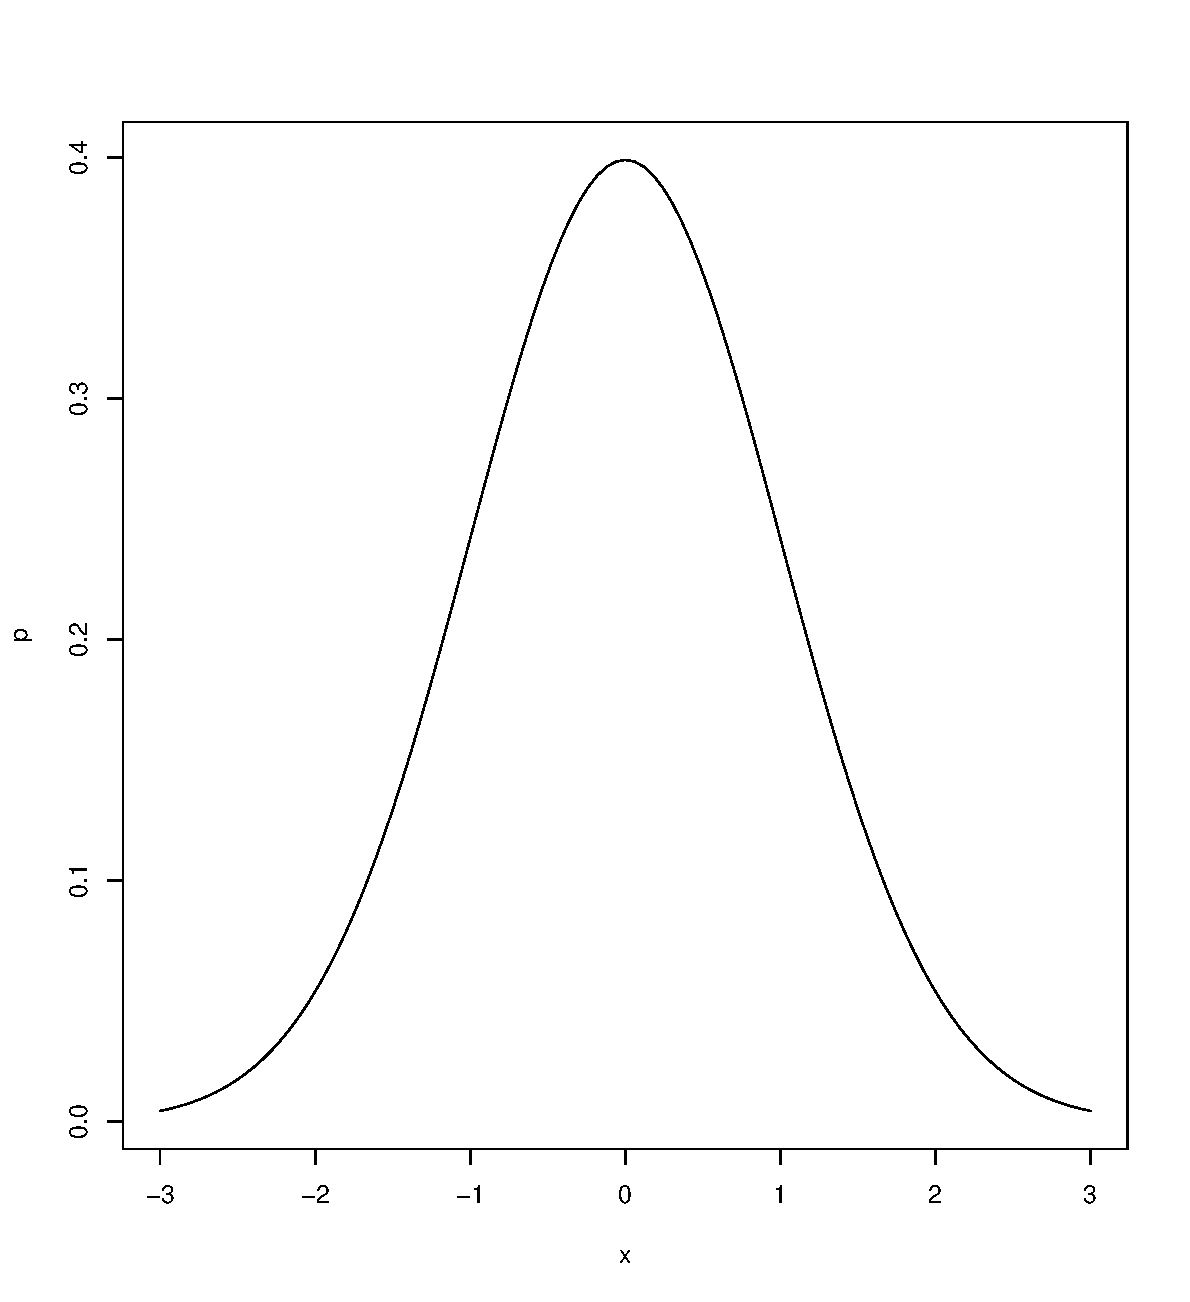
\includegraphics{graphics/plot-normal}
	\label{img:plot-normal}
	\caption{Normal distribution with mean 0 and standard deviation 1.}
\end{figure}

For the purposes of this text it is sufficient to remember the basic properties of the Gaussian distribution. It is a mathematical function of 2 parameters: $\mu$ and $\sigma$. When $\mu = 0$ and $\sigma = 1$ we call the resulting function of $x$ a standard normal distribution. A plot which shows how $P(x)$ varies as $x$ changes is shown in figure \ref{img:plot-normal}. 

If different values are plugged in for $\mu$ and $\sigma$, the shape of the curve will change. By changing $\mu$, the curve can be moved left or right. If $\sigma$ is changed, the bell can be made wider and narrower. We write: $X \thicksim N(\mu, \sigma)$ and we say that the random variable $X$ is normally distributed with mean $\mu$ and standard deviation $\sigma$. We can use our estimates for mean and standard deviation of ages in the marathon data: $36.98$ and $11.03$ respectively. With these parameters a plot can be drawn using R:

\begin{Verbatim}
> curve(dnorm(x, mean(ages), sd(ages)), from=0, to=80)
\end{Verbatim}

\begin{figure}
	\centering
	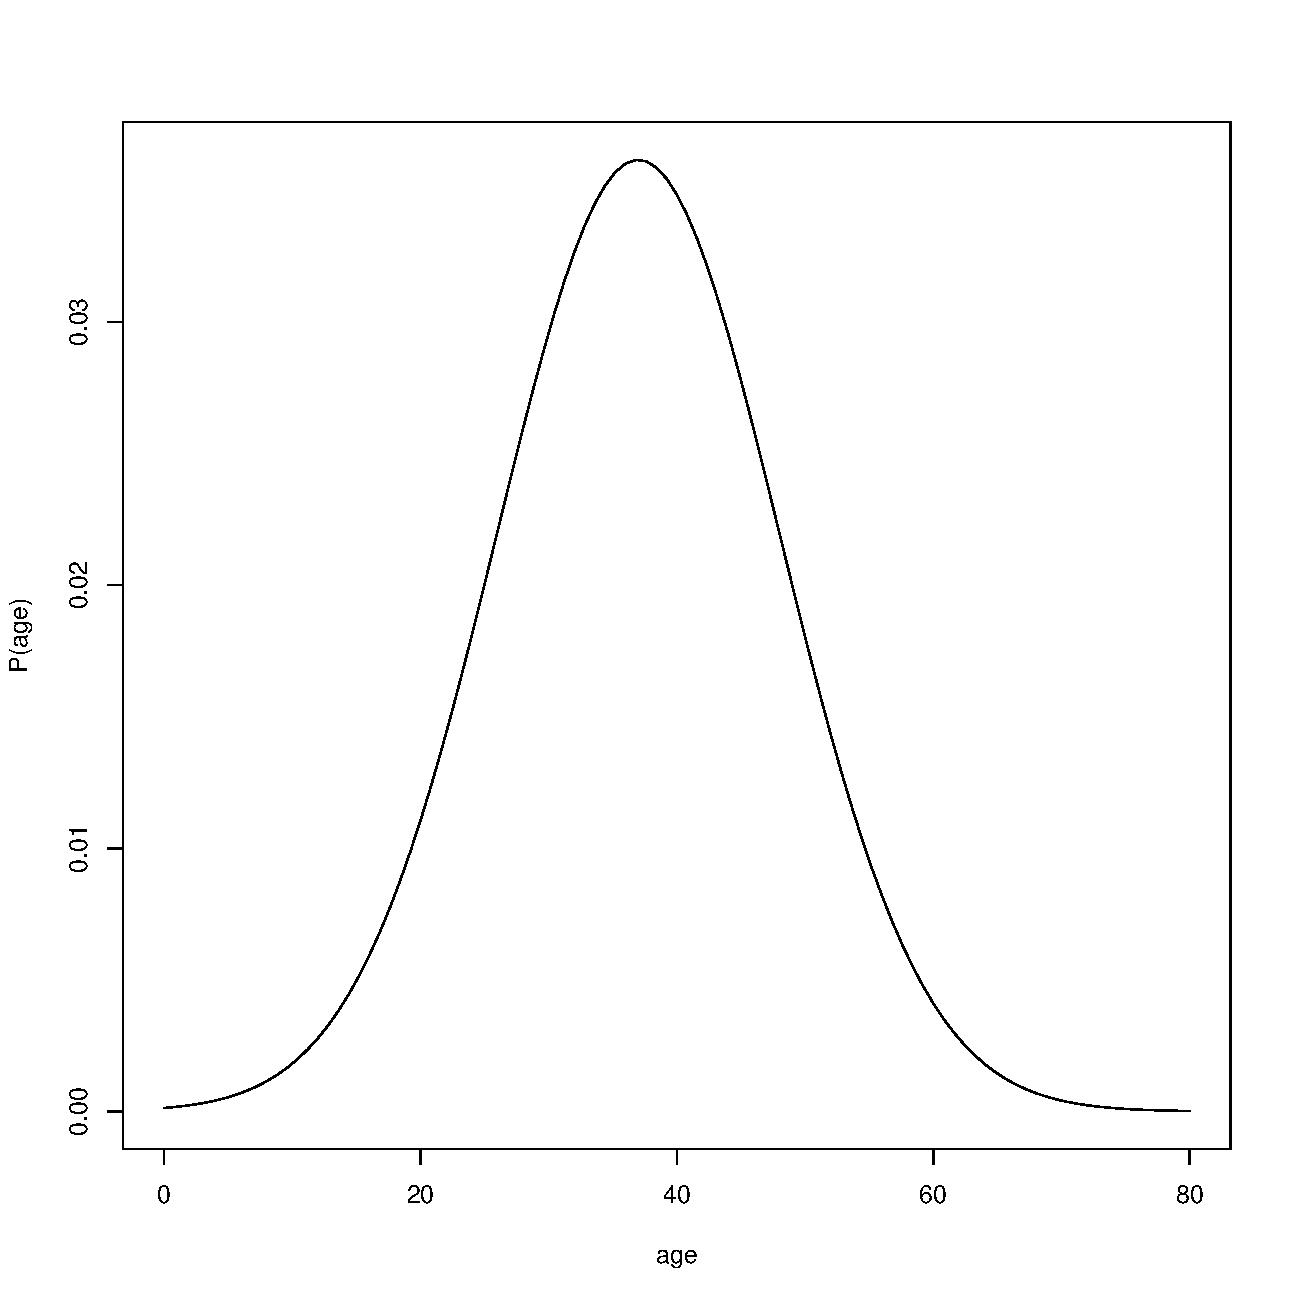
\includegraphics{graphics/plot-curve-ages}
	\label{img:plot-curve-ages}
	\caption{Normal distribution with mean $36.98$ and standard deviation $11.03$.}
\end{figure}

and the result is shown in figure \ref{img:plot-curve-ages}. Thus we have constructed our first mathematical model which shows our guess at how many runners of each age participated in this marathon. The y-axis can be loosely interpreted as the percentage of runners with age x. If the values $P(age)$ for all $x$ are added up, the result is 1 (we added up 100\% of the participants). Another noteworthy property of the function is that if you add up all values $P(age)$ for $0 < x < 20$, the result will be the probability that a runner is under 20 years old. 

Unfortunately the real data does not look like this curve at all and we will explore why and how in the following chapters.

\section{Shape}
In the previous sections on center and spread of data we observed that the robust estimators give different values from the corresponding least squares estimators. So far this was explained by the presence of outliers however this is omitting part of the picture. So far the assumption was that there is an expected value $\mu$, some spread around $\mu$ called $\sigma$ and that the data spreads symmetrically. If the spread is asymmetrical, we say that the data is skewed. The normal distribution model presented in \ref{formula:normal-distribution} accounts only for shifts along the x-axis and changes in the bell width, skewness is not accounted for. This means that if the data is skewed, it cannot be modeled using a normal distribution. Examples of skewed curves are shown in figure \ref{img:skewness}.

\begin{figure}
	\centering
	\includegraphics[trim={4cm 3cm 4cm 5cm},clip]{graphics/skewness}
	\label{img:skewness}
	\caption{Effect of positive and negative skewness.}
\end{figure}

Skewness\cite{Doane2011} can also be estimated using a least mean squares estimator. In order to gain an understanding of how the estimator works, it is useful to introduce the notion of ``central moments''. Central moments are statistics which describe the centrality of data. The first and second central moment have already been covered in depth -- they are mean and variance. Informally, the number (first, second, third, ...) corresponds to the degree at which the error term is raised. 

With this understanding it may be easier to grasp the measure for skewness shown in equation \ref{formula:skewness} - it is a ratio of the third $m_3$ and second $m_2$ moments. $m_2$ is raised to the power $3/2$ so that it is on the same scale of units (cubic) as the third moment. 

\begin{equation} \label{formula:skewness}
	g_1 = \frac{m_3}{m_2^{3/2}} = 
	\frac{\frac{1}{n}\sum_{i=1}^{n}(x_i - \bar{x})^3}
	{\Big[\frac{1}{n}\sum_{i=1}^{n}(x_i - \bar{x})^2\Big]^{3/2}}
\end{equation}

Skewness is not built into the R language, however as is often the case, it can be added by installing an additional R package. I have used the package {\em e1071} and calculated the skewness of ages in the marathon data as:

\begin{Verbatim}
> skewness(ages)
[1] 0.5876703
\end{Verbatim}

The positive value suggests that the data is leaning to the left meaning that there are more younger runners than older runners. This result is a first hint that the data might not be normally distributed. Whether it can be modeled with a normal distribution depends on how strongly it deviates from the bell curve.

Note that the error term is raised to the third power which makes the statistic even more sensitive to outliers than variance. While a robust version of the estimate for skewness called medcouple\cite{Brys2004} exists, it is  too complex to cover here.

Very briefly and for the sake of completeness the fourth central moment is covered: kurtosis. The measure for kurtosis in equation \ref{formula:kurtosis} is a ratio between the fourth and second central moments. Note that $m_2$ is already squared so raising it to the second power brings it onto the same scale as $m_4$. Intuitively speaking, kurtosis is a measure for how pointy the bell curve is. A positive value indicates that the apex is sharper than that of the normal distribution and a negative value indicates a flatter top.

\begin{equation} \label{formula:kurtosis}
	g_2 = \frac{m_4}{m_2^{2}} = 
	\frac{\frac{1}{n}\sum_{i=1}^{n}(x_i - \bar{x})^4}
	{\Big[\frac{1}{n}\sum_{i=1}^{n}(x_i - \bar{x})^2\Big]^{2}}
\end{equation}

Using the R package {\em e1071} the kurtosis of ages in the marathon data can be calculated as:

\begin{Verbatim}
> kurtosis(ages)
[1] -0.1001417
\end{Verbatim}

indicating that the distribution falls off faster around the center than a normal distribution. Of course the measure is highly sensitive to outliers which means that the value should be taken with a grain of salt. Unfortunately I am not aware of a robust estimator.


\chapter{Presenting Data}
\label{ch:presenting-data}
Data can be described in four different ways: 

\begin{enumerate}
	\item table
	\item number
	\item text
	\item picture
\end{enumerate}

In the previous two chapters the marathon data was discussed with the help of tables (figure \ref{tab:marathon-data}), numbers (central moments, median, IQR,...) and with text (filling the gaps between figures). This chapter expands upon the fourth way to present data: by using graphs.

\section{Bar Plot}
One of the simplest graphical representations of data is the bar plot. It is used when comparing the size of groups within the data. In figure \ref{img:barplot-genders} a bar plot is used to compare the number of men to the number of women who participated in the 2016 San Francisco marathon. 


\begin{figure}
	\centering
	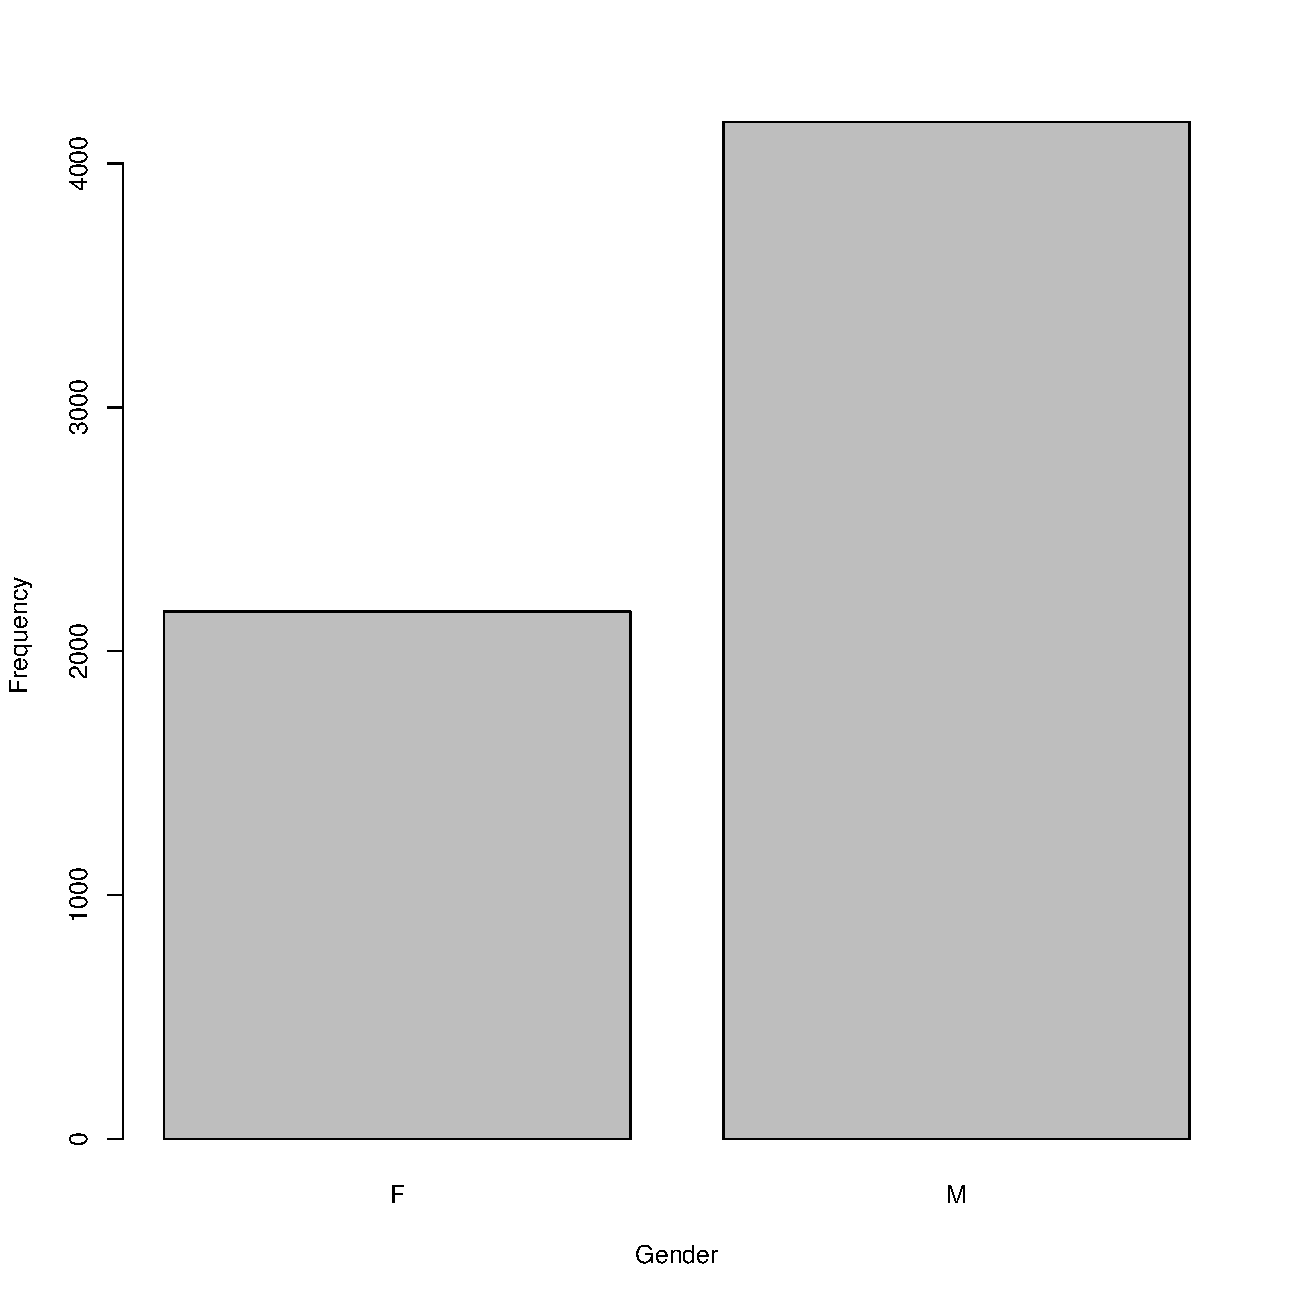
\includegraphics{graphics/barplot-genders}
	\label{img:barplot-genders}
	\caption{Bar plot of participant genders.}
\end{figure}

While the comparison can be easily expressed as a table: 

\begin{Verbatim}
> table(genders)
genders
F    M 
2163 4171 
\end{Verbatim}

the tabular representation requires the reader to read the numbers and perform some mental arithmetic before drawing the conclusion that roughly twice as many men participated.

\begin{figure}
	\centering
	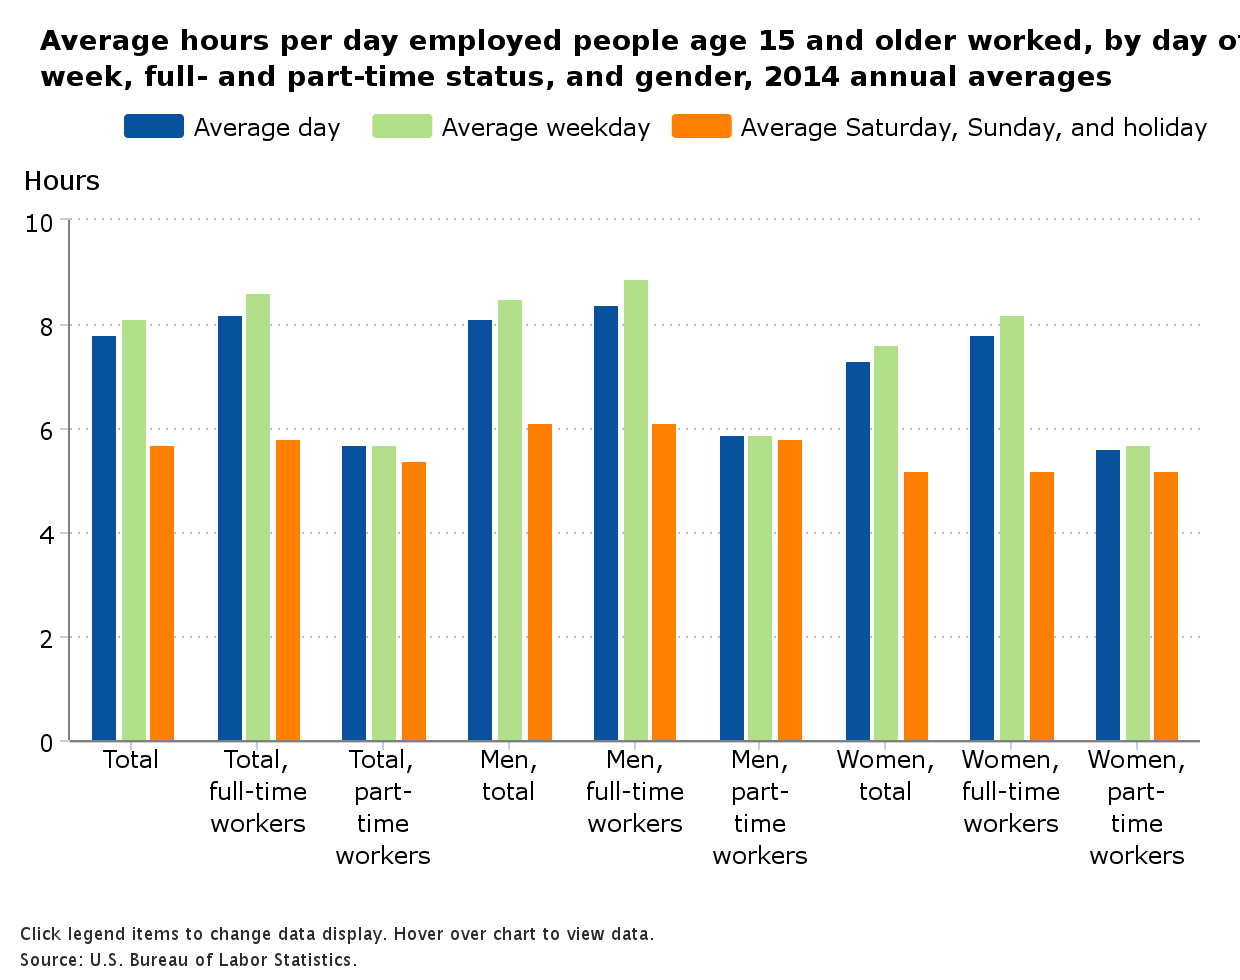
\includegraphics{graphics/average-hours-worked}
	\label{img:average-hours-worked}
	\caption{Average hours per day employed people age 15 and older worked, by day of week, full- and part-time status, and gender, 2014 annual averages.}
\end{figure}

While a bar plot has merits, mainly that it uses our brain's pre-programmed ability to think ``this is bigger than that'', it is sometimes pushed beyond the limits of its usefulness. 

One example is the US Department of Labor's attempt to compare the hours spent working by men and women\footnote{\url{https://goo.gl/25XzTn}}. 
\begin{tcolorbox}
The lesson learned from the bureau's bar plot is: never use a graph to demonstrate more than one point. Our brains can quickly compare the size of two bars however they are not very good at processing more than 3-4 items at the same time. Comparing 27 bars at the same time is a challenge even for experienced data analysts. 
\end{tcolorbox}
Of course the Department of Labor also produces other graphs which are excellent!\footnote{\url{https://goo.gl/lJ463D}}

\section{Histogram}
A close cousin of the bar plot is the histogram. While bar plots and histograms look very similar, they are fundamentally different. Bar plots compare distinct groups under the assumption that there is no meaningful data between these groups. Histograms on the other hand represent the distribution of data on a continuous scale. The two plots can be distinguished by the gaps between bars which are present in bar plots but missing in histograms.

\begin{figure}
	\centering
	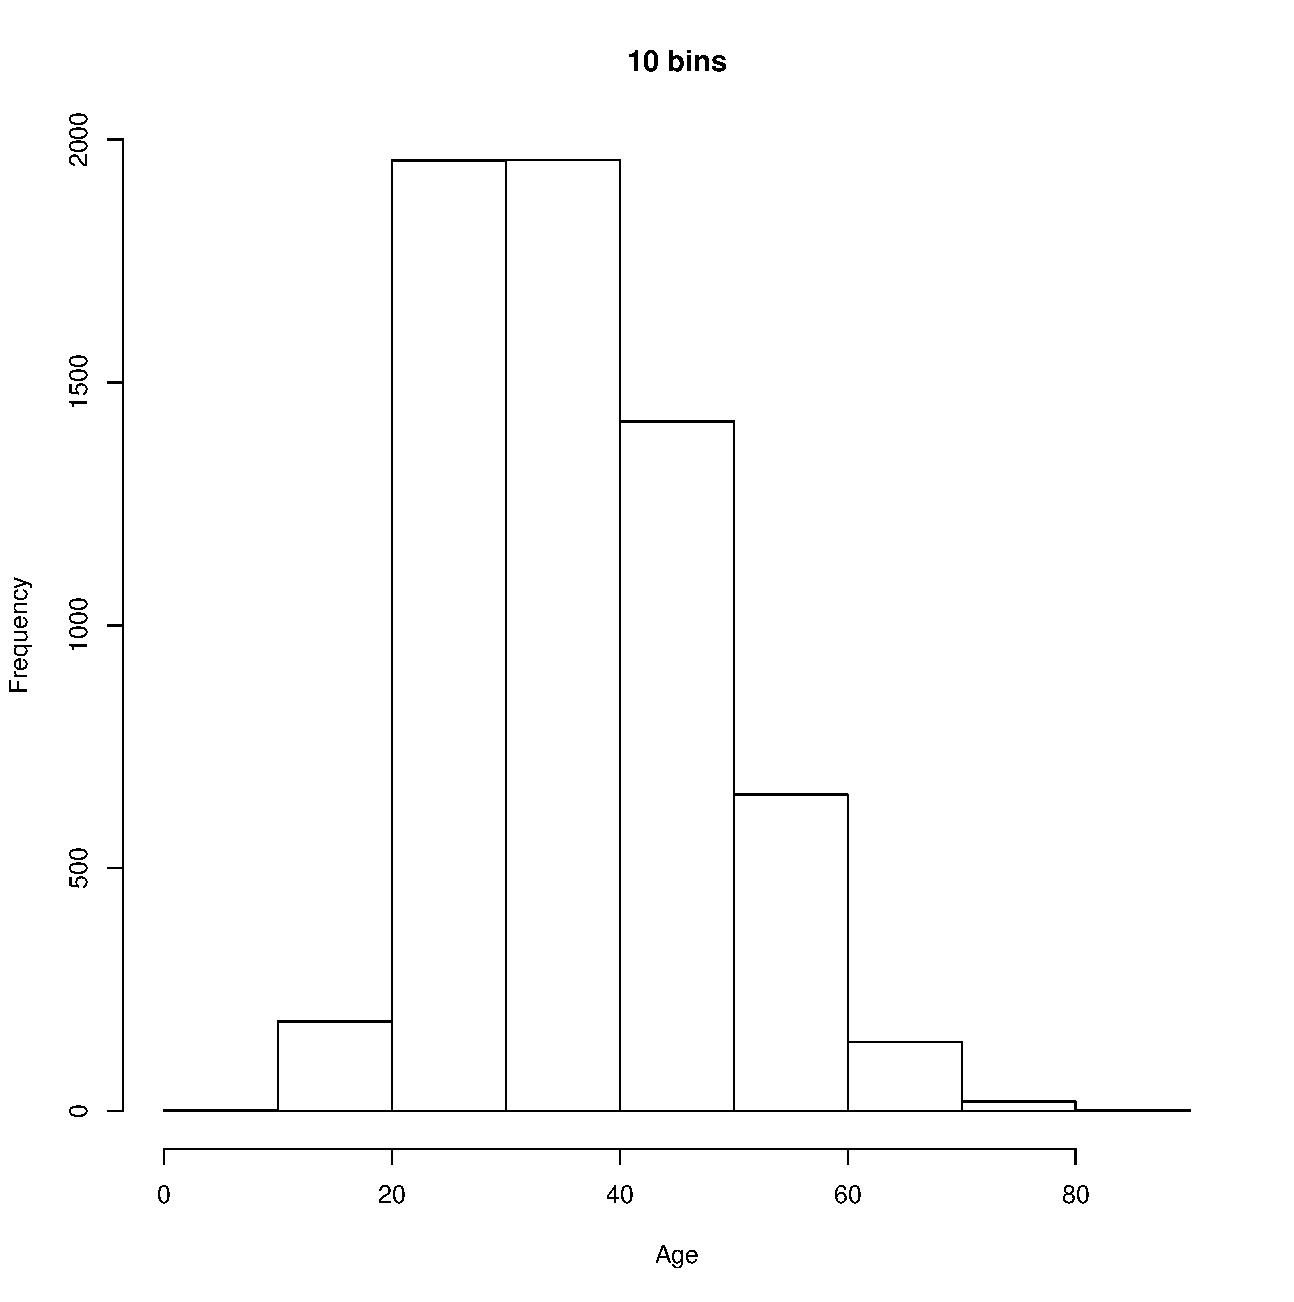
\includegraphics{graphics/histogram-ages-10bins}
	\label{img:histogram-ages-10bins}
	\caption{Histogram of ages.}
\end{figure}

To create a histogram the data is split into equally sized bins. A bar is drawn which corresponds to each of the bins. Taller bars express that more observations fall into the bin. Figure \ref{img:histogram-ages-10bins} shows a histogram of ages in the marathon data. In this graph we can finally see the shape which we have been trying to infer with summary statistics in the previous chapter. While the level of detail is fairly crude, it can be seen that the center lies somewhere between 20 and 40. The corresponding summary statistics were the mean at 36.98 and the median at 35. It is also visible that the ``bell'' is not symmetrical. On the left side is a steep cliff while the right side is a gentle walk down -- this reflects the skewness value of 0.58.

\begin{figure}
	\centering
	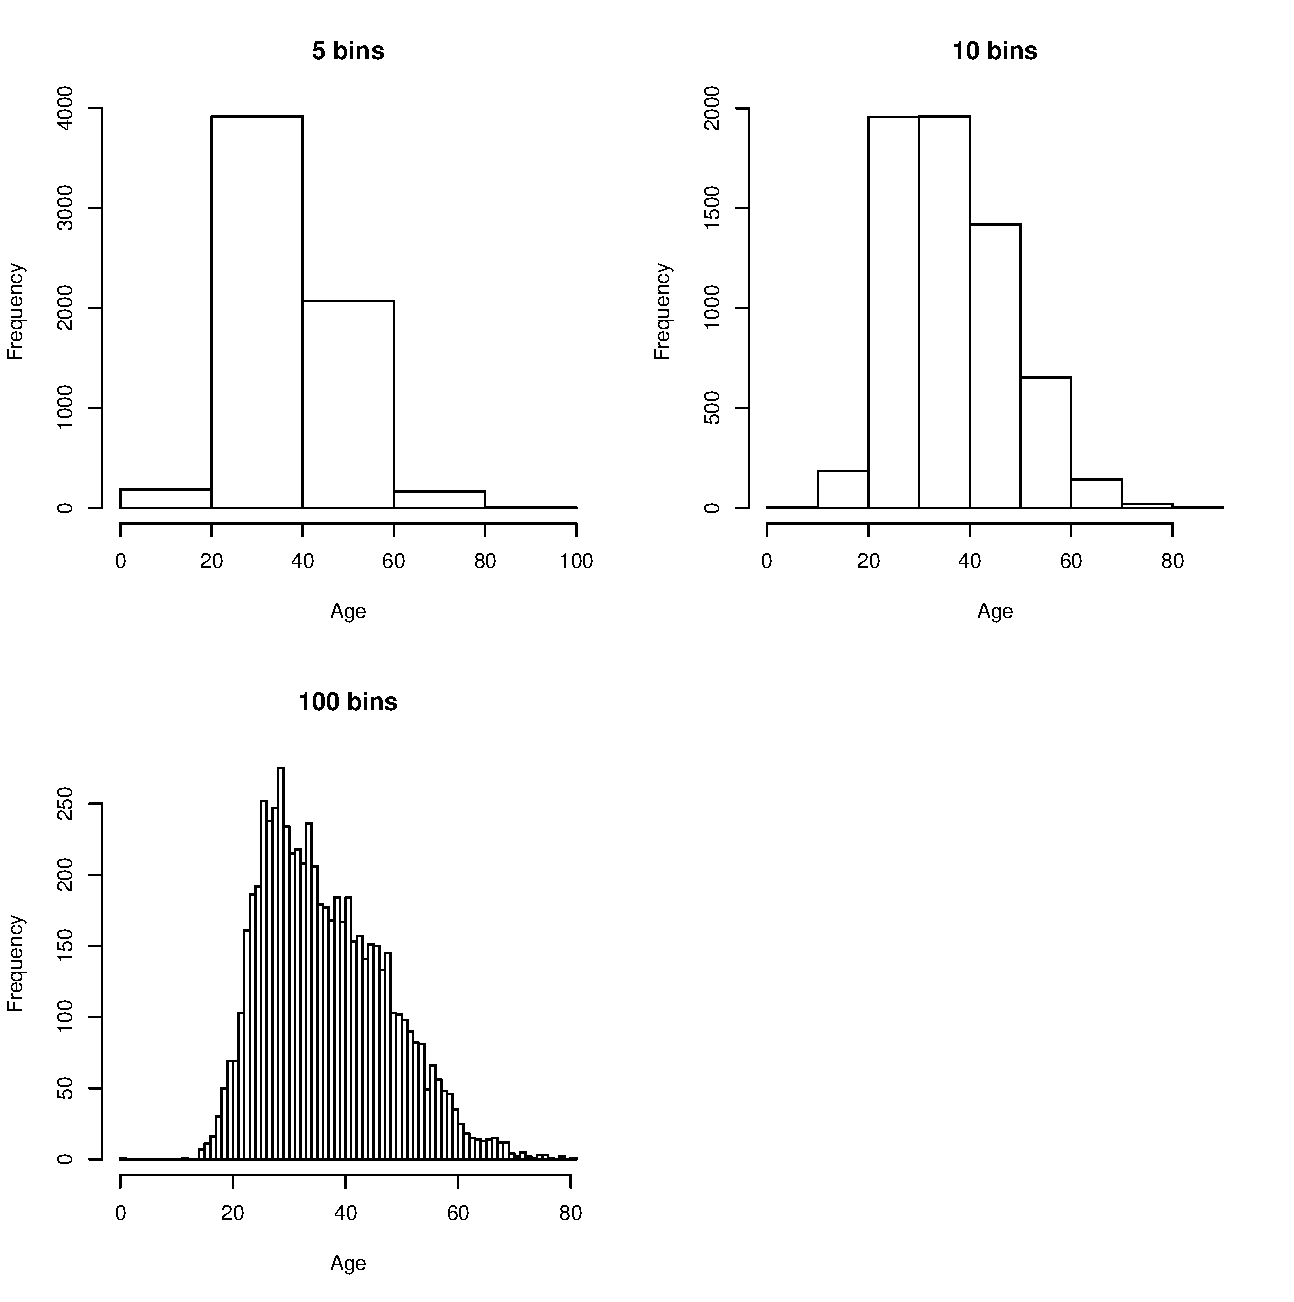
\includegraphics{graphics/histogram-ages-allbins}
	\label{img:histogram-ages-allbins}
	\caption{Histograms of ages with different bin sizes.}
\end{figure}

The difficulty with histograms is choosing the right number and size of bins into which to split the data. Using too few bins would obscure patterns in the data. Choosing a number of bins that is too large on the other hand would reveal detail which is due to variation in the data and is not systematic. Figure \ref{img:histogram-ages-allbins} shows three different histograms of the same data (ages of marathon runners) split into 5, 10 and 100 bins. The 5 bin histogram treats 5 to 20 year olds the same. When using 10 bins, it becomes clear that thankfully there were no runners under 10 years of age. If the data is split into 100 bins however, a lone 0 year old runner appears on the left side of the graph. This is not a super-human toddler but simply a runner who's age was not recorded for some reason.

\section{Box Plot}
Box plots\cite{tukey1977}, sometimes called box and whiskers plots, were invented by John Tukey. Coincidentally, he is also said to have coined the term ``bit'' (short for binary digit) as measure for information. 

\begin{figure}
	\centering
	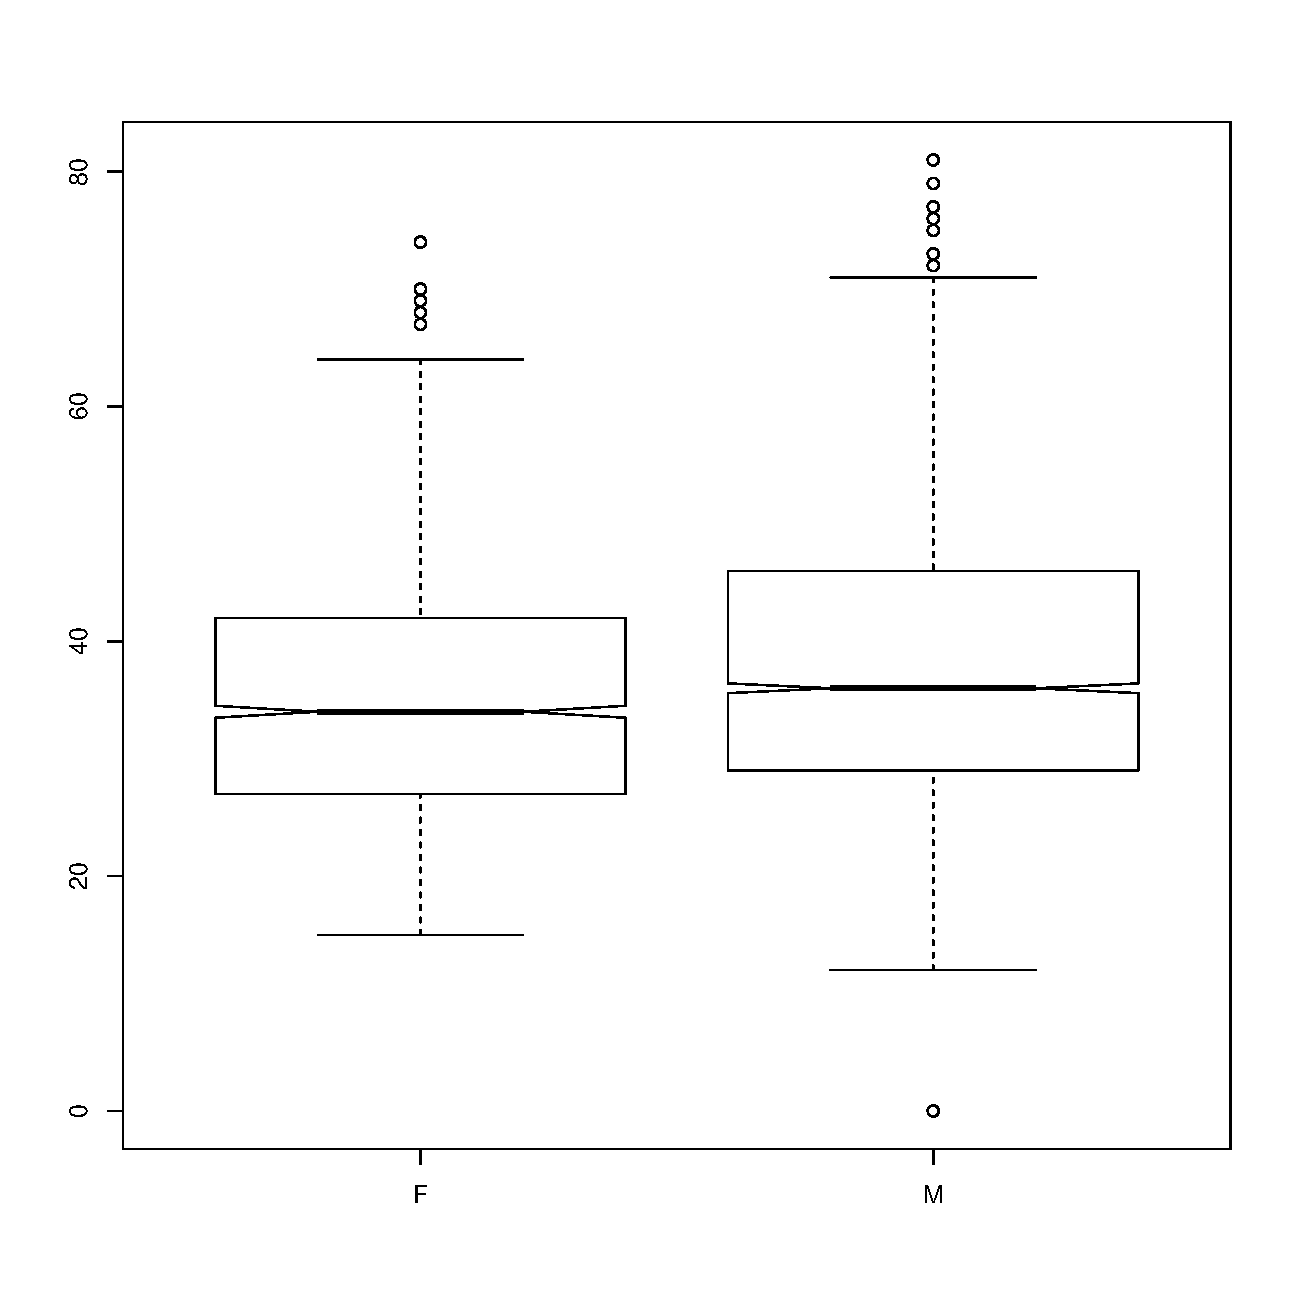
\includegraphics{graphics/boxplot-age-gender}
	\label{img:boxplot-age-gender}
	\caption{Box plot comparing the age of runners between genders.}
\end{figure}

Figure \ref{img:boxplot-age-gender} shows two box plots which compare the age of runners between the genders. This is in essence a graphical representation of robust measures for centrality. The bottom and top edge of the box correspond to the IQR: 50\% of data are in the box. Across the box is a line which shows the median. Above and below of the box stretch a pair of whiskers which depict the range of values which covers 90\% of data. In this framework, data in the top or 5\% are considered outliers.

The notches\cite{chambers1983} which cut into the box are a representation of confidence about whether the medians of two box plots are same or different. If the notches overlap, it is interpreted as strong evidence (95\% confidence) that the medians do not differ. The top and bottom of the notch is calculated as $+- 1.57 \times IQR /  \sqrt{n}$.

In the context of ages, the graph in figure \ref{img:boxplot-age-gender} is showing that while male runners were some of the youngest, overall they were the older group.

\section{Scatter Plot}

\begin{figure}
	\centering
	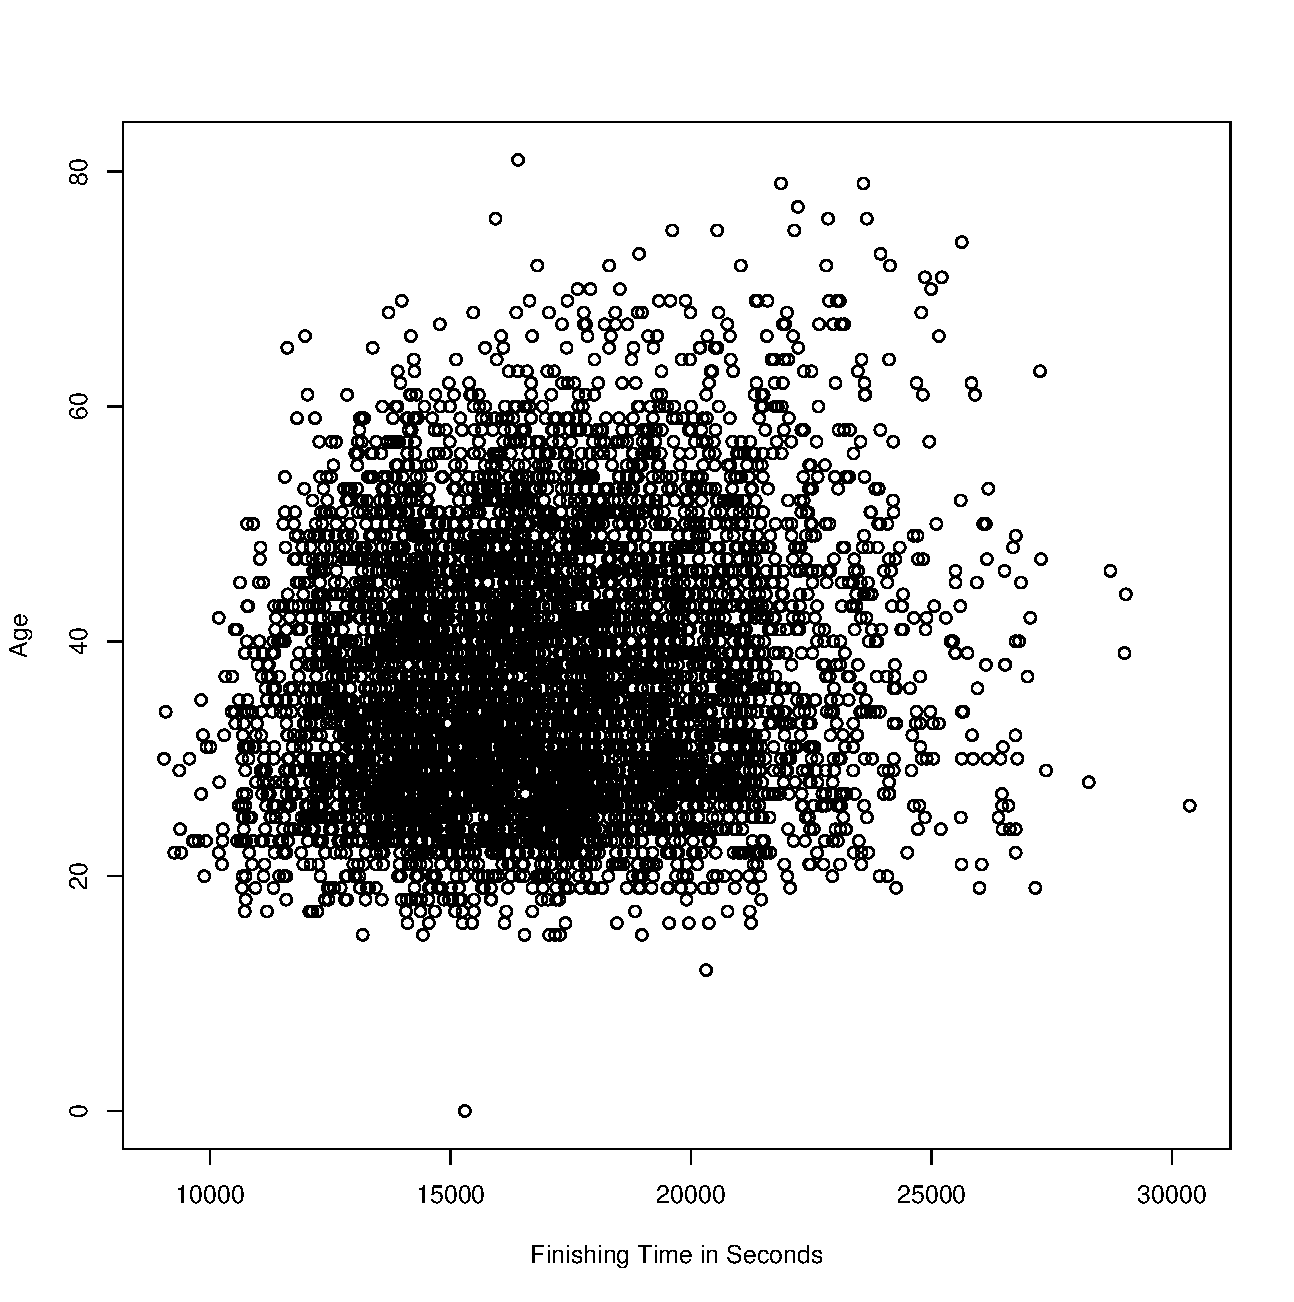
\includegraphics{graphics/plot-age-time}
	\label{img:plot-age-time}
	\caption{Correlation of age and finishing time.}
\end{figure}

\begin{figure}
	\centering
	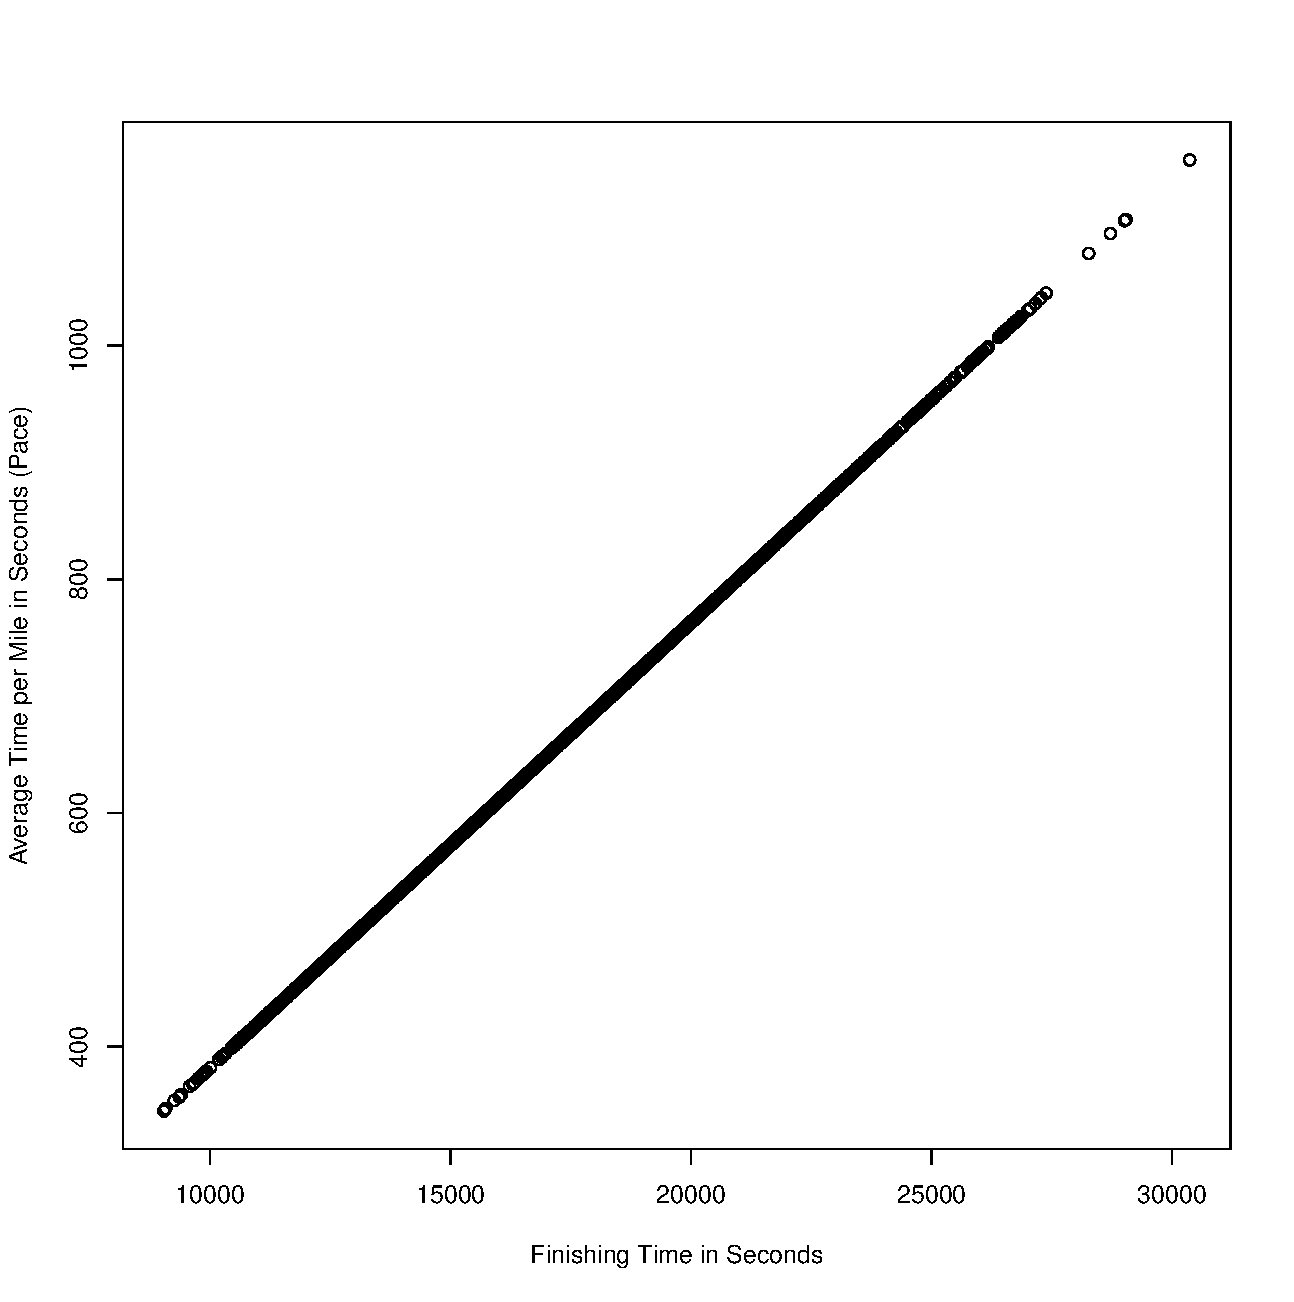
\includegraphics{graphics/plot-pace-time}
	\label{img:plot-pace-time}
	\caption{Correlation of pace and finishing time.}
\end{figure}

Probably most frequently seen in scientific articles, is the scatter plot. Its purpose is to visualize how one variable changes in relation to another. The scatter plot in figure \ref{img:plot-age-time} shows how the finishing time of runners changes in relation to their age (or vice versa). What can be seen in the graph is that while the most competitive runners are under 40, for the vast majority of data no apparent pattern is visible which could explain finishing times as a function of age. In contrast, figure \ref{img:plot-pace-time} shows the relation between pace and finishing time. Pace is the time a runner took per mile. This graph shows a very strong correlation between the two variables -- I would wager that knowing one piece of information the other can be predicted 100\% accurately. The reason for this is hardly clairvoyance, more than likely pace is calculated at the end of a race by dividing a runner's finishing time by the number of miles in a marathon.

\begin{tcolorbox}
	Guidelines for creating legible graphs:
	\begin{itemize}
		\item Illustrate one point per graph.
		\item Use an appropriate visualization method. For example don't use a bar plot when you are showing a histogram.
		\item Include a title which clearly explains the contents of your graph.
		\item Variables visualized along an axis must be clearly labeled.
		\item The scale of axes must be labeled with equidistant tick marks. If your data is exponential, it is usually better for understanding to transform the data logarithmically than to change the distance between tick marks.
		\item The range of axes must have no interruptions. If the lowest value is 0 and the highest 10,000, all values in between must be visualized on the graph.
		\item If you are comparing two graphs next to each other, the scale and range of axes on both graphs must be the same.
		\item The font size of graphs must be the same as the font size of text around the graph.
	\end{itemize}
	
	This list is not exhaustive. When in doubt, keep it simple and ask friends to try and interpret your graph.
\end{tcolorbox}
\chapter{Asking Questions}
The methods presented thus far all had one thing in common: describing the shape of data. This can be done graphically or by interpreting summary statistics such as arithmetic mean and standard deviation.

In this chapter, a different approach to analyzing data is presented. In this new approach the theoretical notion of probability is connected with the data observed in reality. The recurring question in this chapter will be: To what extent does the observed data represent the set of data it was drawn from? The answer to this question is arrived at in three steps:

\begin{enumerate}
	\item form a hypothesis $H_0$
	\item model probability of $H_0$ being observed
	\item conclude probability of $H_0$ being valid as a function of observed data
\end{enumerate}

A hypothesis, in layman's terms, is a question about the data. An example of such a question is: ``Is the mean age of marathon runners different from 30?''. The question is then answered in step 3 of the method. Step 2 is fairly complex and far outside the scope of an introduction to statistics. Fortunately probabilistic models for many useful questions that can be asked of data have already been created by other, more experienced statisticians. These models can be used without change long as the questions we ask follow the paved path.

\section{Statistical Testing}
While forming probabilistic models from scratch is usually an arduous adventure, we can create a model to answer a simple question to illustrate the fundamental concepts.

The question in the previous section about whether the mean of marathon runners is different from 30 was chosen deliberately. The reason for this phrasing is that it fits a method designed to answer questions of the form $H_0: \mu = \mu_0$ where $\mu$ is the mean of the underlying distribution and $\mu_0$ a number we are interested in as a potential candidate for being equal to $\mu$. The method in question is called the \hbox{Z-Test} and is essentially a formula which given data produces the probability of $H_0$ being observed:

\begin{equation}
P(H_0 = True) = \hbox{Z-Test}(data)
\end{equation}

To build an understanding of why and how this process works, it is helpful to recall our previous discussion of the arithmetic mean. Equation \ref{formula:arithmetic-mean} in the last chapter shows an estimator for the true mean. Importance is placed here on the difference between the true mean, a parameter of the underlying distribution, and the estimated mean, a function of the observed data. We also noted that when we observe a different sample of data from the same distribution, the estimate would also change. In other words, if we take 3 different sub-samples of 100 marathon runners and calculate the mean of each group, we would expect the means of all 3 groups to be reasonably similar but different. It would seem that since the means are estimated by observing a random variable, the means themselves can be treated as a random variable. 

For the sake of argument, let us assume that the ages of runners are normally distributed. What would be the distribution from which the estimated mean age is drawn? An exhaustive and rigorous answer to this question would take us deep into the territory of calculus and theory of probability. Here we will limit ourselves to an intuitive argument which makes the connection between theoretical distribution and observed data more apparent.

Two leaps of faith are made to simplify this explanation: firstly, the arithmetic mean estimator when used on normally distributed data is itself distributed normally: $\bar{X} \thicksim N(\mu_{\bar{X}}, \sigma_{\bar{X}})$. The expected value of $\mu_{\bar{X}}$ coincides with the value of expectation for $\mu$ of the underlying data. Our second leap of faith is needed to derive the variance of $\mu_{\bar{X}}$:

\begin{equation}
Var(\bar{X}) = Var(\frac{1}{n}\sum_{i=0}^n X_i)
\label{formula:mean-variance}
\end{equation}

Keen observation reveals that in order to come up with a variance for $\bar{X}$ we treat the arithmetic mean estimator as a function of $X_i$. The parameter $X_i$ represents not as per usual our observed data but the slightly different notion of $n$ random variables coming from the same distribution as the observed data. This subtle distinction signifies that we are making an assumption about the distribution of observed data. Knowing the assumptions implicitly made by a statistical method is crucial to producing accurate results. If your experiment violates the assumptions, your results will be meaningless. In this case there are three assumptions:

\begin{enumerate}
	\item $X$ is normally distributed
	\item the observations of all $X_i$ are independent of each other
	\item the population variance exists and is known
\end{enumerate}

Assumption 2 leads directly to the second leap of faith necessary to conclude formulating the \hbox{Z-Test}. When the $X_i$ are independent the following property holds for their variances  \footnote{\url{https://en.wikipedia.org/wiki/Variance}}:

\begin{equation}
Var(\sum_{i=0}^n a X_i) = a^2 \sum_{i = 0}^n Var(X_i)
\label{formula:variance-property}
\end{equation}

Using the property in equation \ref{formula:variance-property} the variance of $\bar{X}$ defined in equation \ref{formula:mean-variance} can be expanded as:

\begin{equation}
Var(\bar{X}) = Var(\frac{1}{n}\sum_{i=0}^n X_i) = \frac{1}{n^2}\sum_{i=0}^n Var(X_i) = \frac{\sigma^2}{n}
\end{equation}

to arrive at the distribution of the arithmetic mean $\bar{X} \thicksim N(\mu, \frac{\sigma^2}{n})$. This would be sufficient to test our hypothesis $H_0: \mu = 30$. In textbooks however you will find a different definition of the \hbox{Z-Test}:

\begin{equation}
Z = \frac{\bar{X} - \mu}{\sigma / \sqrt{n}}
\label{formula:z-test}
\end{equation}

The reason for this formulation of the test is historical. Before computers were commonly available, it was notoriously difficult to compute probabilities for given distributions and values. So difficult in fact that in the back of most statistical textbooks one could find tables of precomputed probabilities. These were provided only for common distributions such as $N(0, 1)$. The $Z$ value in equation \ref{formula:z-test} is simply a reformulation of the statistic in such a way that $Z \thicksim N(0, 1)$.

Here we will use R instead of printed out tables to answer the question whether the average age of runners is significantly different form 30. If we would like to be 95\% certain of our answer, that is almost certainly certain, we use the R function {\em qnorm} to figure out the top and bottom 2.5\% of the distribution -- the most unlikely values. The actual $\mu$ is 95\% likely to be between those boundaries.

\begin{verbatim}
> qnorm(0.025, mean(ages), sd(ages) / sqrt(length(ages)))
[1] 36.71596
> qnorm(1-0.025, mean(ages), sd(ages) / sqrt(length(ages)))
[1] 37.2594
\end{verbatim}

We conclude that any estimates of the average age lower than 36.71596 and above 37.2594 are extremely unlikely to occur. The value 30 is certainly deep inside the critical region of our test. We say that $H_0$ is rejected which means that the alternative hypothesis $H_1: \mu \neq 30$ holds and we are 95\% confident. 

At this point it is worth remembering that the ages of marathon runners are not normally distributed which violates assumption 1 of the test and renders our finding meaningless.

\begin{tcolorbox}
	The key take-aways from this section are:
	\begin{itemize}
		\item Form a null hypothesis $H_0$ and an alternative hypothesis $H_1$ to fit an existing test.
		\item Know the assumptions of the test you are planning to use and verify that you are not violating any of them.
		\item Your statistical software of choice will return the probability of the test statistic (e.g. $Z$) occurring (p-value).
		\item If the p-value is low $p<0.05$, $H_0$ is rejected with confidence $1 - \hbox{p-value}$. Otherwise $H_0$ cannot be rejected.
	\end{itemize}
\end{tcolorbox}

\section{Test for Normality}
In the previous section we introduced a language in which to ask questions that can be answered with statistical tests. The \hbox{Z-Test} is just one of hundreds other methods which are cataloged in literature\cite{kanji2006} and ge be drawn upon as needed. In addition, most of the tests are already implemented in the R software package so even the tricky nature of implementing mathematical methods in software can be avoided. A point stressed in the context of the \hbox{Z-Test} is that it only works as expected if the data is drawn from a normal distribution. 

Fortunately there is a statistical test which can be used to check if the data comes from a normal distribution. The null hypothesis $H_0$ is ``the difference an observed and a specified distribution is not significant'' with $H_1$ implying that the two distributions are significantly different. The assumption made by the test is that both probability distribution functions are continuous.

For this experiment we will depart from the ages of runners and compare their finishing times instead. The first comparison is of times between genders:

\begin{Verbatim}
> ks.test(allTimes[genders == 'M'], allTimes[genders == 'F'])

Two-sample Kolmogorov-Smirnov test

data:  allTimes[genders == "M"] and allTimes[genders == "F"]
D = 0.19616, p-value < 2.2e-16
alternative hypothesis: two-sided
\end{Verbatim}

The \hbox{p-value} is very close to zero meaning that it is very unlikely the finishing times for ladies and gents were drawn from the same distribution. Tests presented in the following sections which compare the means and variances of two groups assume that the data is distributed normally. If we would like to have meaningful results, we need to ensure that the finishing times of both genders are normally distributed. The Kolmogorov Smirnov test can be used to check this assumption:

\begin{Verbatim}
> ks.test(allTimes[genders == 'M'],
+     pnorm,
+     mean(allTimes[genders == 'M']),
+     sd(allTimes[genders == 'M']))

One-sample Kolmogorov-Smirnov test

data:  allTimes[genders == "M"]
D = 0.046776, p-value = 2.368e-08
alternative hypothesis: two-sided
\end{Verbatim}

In this case too the \hbox{p-value} is quite small -- certainly far smaller than the usually accepted significance threshold of 0.05. This puts us in an awkward situation which is encountered frequently in data analysis: we would like to perform some tests but our data violates the basic assumptions made by the methods. If we cannot model the data with a function, all methods based on functional analysis of probability distribution functions are meaningless. One way around this limitation is to use so called non-parametric tests which don't assume that the data was drawn from a specific distribution. An example of a non-parametric method for comparing the means of two groups are the box plot notches presented in the previous chapter.

In this chapter however a cheat is introduced which helps get around the non-normal distribution of finishing times. Instead of using the original data, we will use the estimates for mean and variance to generate data which we are certain is normally distributed. The function {\em rnorm} in R can be used to simulate normally distributed data of any size given a value for mean and standard deviation. The following call will return an array of simulated finishing times which are distributed normally:

\begin{Verbatim}
> rnorm(
+     length(allTimes[genders == 'M']), 
+     mean(allTimes[genders == 'M']), 
+     sd(allTimes[genders == 'M']))
\end{Verbatim}

\section{Comparing Means}
Now that it is ensured the distributions of finishing times are normally distributed we can turn to analytical methods of comparing parameters. First, we will compare the mean finishing time for male and female runners. 

A very frequently used statistical test for comparing the means of two groups is Student's \hbox{t-test}\cite{student1908}. The test is over 100 years old dating back to 1908 and has an interesting back story. The author's name is not actually Student but William Gausset. He studied chemistry and mathematics at Oxford and as a top graduate in both was offered to work for the Guiness brewery. While working there William developed this test to monitor the quality of stout -- presumably Guiness. In 1908, much like today, his work was technically owned by Guiness which is why he published under the pseudonym Student (not to be confused with the word ``student''). For one reason or another Guiness didn't go after him with the full might of their legal department and a hundred years later we are still using Student's \hbox{t-test}.

The \hbox{t-test} is part of the core R functionality. We can compare the mean finishing times of runners as follows:

\begin{Verbatim}
> t.test(
+     normalTimes[normalGenders == 'M'], 
+     normalTimes[normalGenders == 'F'])
+ 

Welch Two Sample t-test

data:  normalTimes[normalGenders == "M"] and normalTimes[normalGenders == "F"]
t = -17.489, df = 4568, p-value < 2.2e-16
alternative hypothesis: true difference in means is not equal to 0
95 percent confidence interval:
-1591.534 -1270.679
sample estimates:
mean of x mean of y 
16478.7   17909.8 
\end{Verbatim}

Note that we are comparing the means of simulated data because our original data is not normally distributed. This is an issue Gausset discusses on the very first page of his seminal paper. He argues that if we have a large amount of data available we can perform precise calculations rendering the limitation of needing a normal distribution moot. If however the sample size is small, as is often the case in micro-biological fields such as a brewery, the assumption that the data was drawn from a normal distribution is a guess that is more reasonable than many. 

Occasionally you may need to compare the means of more than two groups. In those cases there are two options: either perform pair-wise t-tests between all groups or opt for an analysis of variance (ANOVA) test. An analysis of the variance of two groups is equivalent to a t-test and can be computed in R as:

\begin{Verbatim}
> fit <- lm(formula = normalTimes ~ normalGenders)
> anova(fit)
Analysis of Variance Table

Response: normalTimes
                Df     Sum Sq    Mean Sq F value    Pr(>F)    
normalGenders    1 2.9172e+09 2917174891  296.49 < 2.2e-16 ***
Residuals     6332 6.2301e+10    9839009                      
---
Signif. codes:  0 `***' 0.001 `**' 0.01 `*' 0.05 `.' 0.1 ` ' 1
\end{Verbatim}

The first step of the analysis is fitting a model which explains the finishing times as a linear function of gender. Linear models and analysis of variance are topics which warrant a chapter of their own (possibly in a future text) which is why we only gloss over them here. In closing, let's use another F-test to compare the variances of finishing times:

\begin{Verbatim}
> var.test(
+     normalTimes[normalGenders == 'M'], 
+     normalTimes[normalGenders == 'F'])

F test to compare two variances

data:  normalTimes[normalGenders == "M"] and normalTimes[normalGenders == "F"]
F = 1.1031, num df = 4170, denom df = 2162, p-value =
0.009329
alternative hypothesis: true ratio of variances is not equal to 1
95 percent confidence interval:
1.024505 1.186677
sample estimates:
ratio of variances 
1.103092 
\end{Verbatim}

The p-value returned by this test is beneath the significance threshold of 0.05 and we conclude that the variance of both groups are different.

\section{Generalization}
A number by itself means little. Unless you know how long it would take you and your friend to run a marathon, it would mean little to you that a runner in the San Francisco 2016 marathon completed the race in just over 2 hours and 30 minutes. Only when you compare this runner's performance to all others will you know that he finished first. To make this conclusion we took one number and compared it to all others within the data. Statistics however starts to really shine when you begin comparing your numbers to things outside your experiment. For example the world records for marathon are currently around 2 hours and 3 minutes which makes the San Francisco winner look slow in comparison.

\begin{figure}
	\centering
	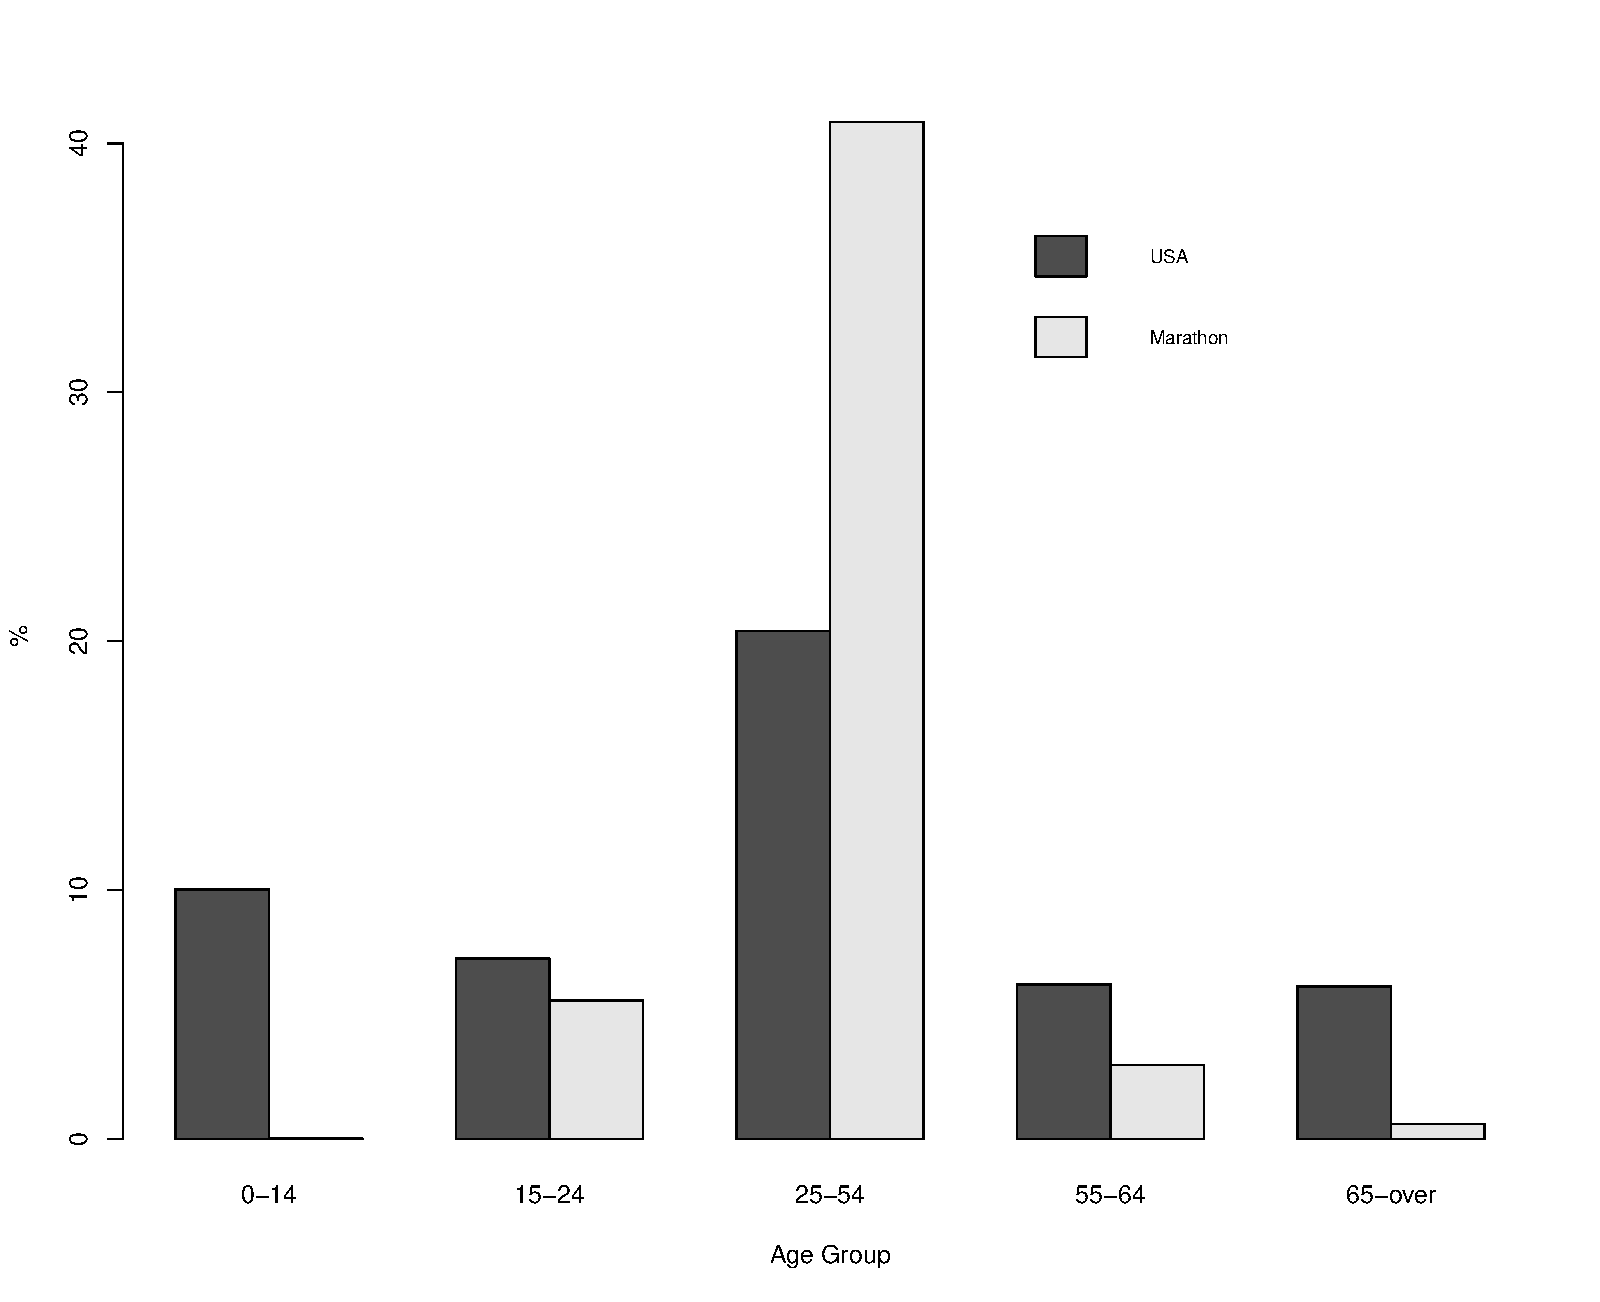
\includegraphics{graphics/barplot-ages-usa-marathon}
	\label{img:ages-usa-marathon}
	\caption{Demographics comparison between USA and Marathon runners.}
\end{figure}

A comparison with the outside world can be made not only for single numbers but also for the distribution of data. Are different age groups in the USA represented equally in the marathon? Figure \ref{img:ages-usa-marathon} gives an initial insight towards answering this question. Often to put your data in a larger context you will need to look for experiments similar to yours. International and national governmental organizations are excellent sources of such data. 

For example to answer the question of age group distribution the data used was collected by the CIA for all countries in the world\footnote{\url{https://www.cia.gov/library/publications/the-world-factbook/fields/2018.html}}. Examples for other trustworthy sources of information are the World Health Organization (WHO), various branches of the United Nations (UN), the World Bank Group, the Program for International Student Assessment (PISA) and many others. You should be suspicious whenever statistics are published by for profit organizations such as private news agencies, pharmaceutical corporations or private financial institutions.

Returning from the political facet of statistics back to figure \ref{img:ages-usa-marathon} we can see that the group of 25 to 54 year olds is over-represented by a factor of 2 at the expense of all other groups. This finding however is subjective as it is based on looking at a picture as opposed to mathematical argument. The keen reader may bring up that the Kolmogorov Smirnov test presented in an earlier section might be used to compare the distribution of ages for the USA and marathon runners. Unfortunately the CIA provides information about age groups in the United States by splitting the range of ages into bins. From this type of information we cannot estimate a continuous distribution function which is a strict requirement of the test.

A statistical test designed to compare discrete (or discretized) distribution functions is the $\chi^2$ test. If you have two groups of data, you can split their numeric range into a number of bins. The $\chi^2$ test can then be used to determine if the difference in number of observations falling into each bin between both groups of data is significant. In very general terms, the squared differences are examined and added in such a way that the result is a number which is drawn from a $\chi^2$ distribution -- hence the name of this test. To compare the age groups of the USA with those of marathon runners we can use R:

\begin{Verbatim}
> chisq.test(comparisonAgeGroups)

Pearson's Chi-squared test

data:  comparisonAgeGroups
X-squared = 3130.7, df = 4, p-value < 2.2e-16
\end{Verbatim}

The function returns three values: a value for the $\chi^2$ test statistic, the degrees of freedom and a \hbox{p-value}. As we already know, the \hbox{p-value} is the probability of observing the value 3130.7 in a $\chi^2$ distribution with 4 degrees of freedom. This probability is very low which is why $H_0$ that both distributions are the same is rejected. Note that here is where the statistical analysis ends. We are very certain that the ratios of age groups in the marathon data are not representative of the United States. This confidence tells us nothing as to the why there is a difference or even what it might mean. 

A newly introduced concept are degrees of freedom. You can treat this as a parameter of the $\chi^2$ distribution which is equal to $n_{bins} - 1$ and not think further of it. If you continue to read about statistics, you will encounter degrees of freedom often which is why it is helpful to have a deeper understanding of this parameter. The number of degrees of freedom is a property of a vector which tells us in how many ways it can be changed. For example the vector 

\begin{equation}
\left(
\begin{array}{c}
X_1 \\
X_2 \\
X_3 
\end{array}
\right)
\end{equation}

can be changed in three ways: along $X_1$, $X_2$ and $X_3$ which is why it has 3 degrees of freedom. With $\bar{X}$ being the sample mean this vector can be decomposed as:

\begin{equation}
\left(
\begin{array}{c}
X_1 \\
X_2 \\
X_3 
\end{array}
\right)
=
\bar{X}
\left(
\begin{array}{c}
1 \\
1 \\
1 
\end{array}
\right)
+
\left(
\begin{array}{c}
X_1 - \bar{X} \\
X_2 - \bar{X} \\
X_3 - \bar{X} 
\end{array}
\right)
\label{formula:decomposition}
\end{equation}

The vector on the left side of the $=$ in equation \ref{formula:decomposition} still has 3 degrees of freedom. The first vector on the right hand side of the equation is defined to be a multiple of the vector $(1, 1, 1)$. It can only change in its length which is why it only has 1 degree of freedom. To understand the degrees of freedom of the last vector bring to mind that $\bar{X}$ is a function of all $X_i$:

\begin{equation}
\bar{X} = \frac{\sum_{i = 0}^n X_i}{n}
\end{equation}

if we set the equation to zero and multiply both sides by $n$ we get the equivalent form:

\begin{equation}
\sum_{i = 0}^n X_i - \bar{X} = 0
\label{formula:constraint}
\end{equation}

How many $X_i$ can be changed without violating equation \ref{formula:constraint}? The first $n-1$ can be varied freely however once they are fixed, the last component must be chosen in such a way that it cancels the sum out to 0. In other words, the last vector in equation \ref{formula:decomposition} has 2 degrees of freedom. As to the $\chi^2$ test statistic, without going into too much detail, the reason for its degrees of freedom is that we are comparing $n$ bins equating to $n$ ways the statistic can move however they are compared as ratios of the total number of observations. Calculating the total predetermines one degree of freedom.



\backmatter

%----------------------------------------------------------------------------------------
%	BIBLIOGRAPHY
%----------------------------------------------------------------------------------------

\bibliography{bibliography} % Use the bibliography.bib file for the bibliography
\bibliographystyle{plainnat} % Use the plainnat style of referencing

%----------------------------------------------------------------------------------------

\printindex % Print the index at the very end of the document

\end{document}